\documentclass[runningheads,a4paper]{llncs}

\documentclass[runningheads,a4paper]{llncs}

\usepackage{graphicx}
\usepackage[space]{grffile}
\usepackage{latexsym}
\usepackage{amsfonts,amsmath,amssymb}
\usepackage{url}
\usepackage[utf8]{inputenc}
\usepackage{textcomp}
\usepackage{longtable}
\usepackage{multirow,multicol,booktabs}
\usepackage{xcolor}
\usepackage{xspace}
\usepackage{amssymb}
%\setcounter{tocdepth}{3}
\usepackage{caption}
\usepackage[caption=false]{subfig}

\bibliographystyle{abbrv} 

\newcommand{\keywords}[1]{\par\addvspace\baselineskip\noindent\keywordname\enspace\ignorespaces#1}
\newcommand{\ceiling}[1]{\left\lceil{#1}\right\rceil}
\newcommand{\floor}[1]{\left\lfloor{#1}\right\rfloor}
\newcommand{\setof}[1]{\left\{{#1}\right\}}
\newcommand{\set}[2]{\{{#1}\mid{#2}\}}
\newcommand{\jj}[1]{\textcolor{blue}{jj: #1 : endjj}}

%%%%%%%%%%%%%%%
 \def\myendproof{{\ \vbox{\hrule\hbox{%
   \vrule height1.3ex\hskip0.8ex\vrule}\hrule }}\par}
 \renewenvironment{proof}{\noindent{\bf Proof. }}{\myendproof}  
  
%\newtheorem{theorem}{Theorem}
%\newtheorem{lemma}{Lemma}
%\newtheorem{corollary}{Corollary}
%\newtheorem{example}{Example}
%\newtheorem{claim}{Claim}
%\newtheorem{definition}{Definition}
%\newtheorem{rrule}{Rule}
%\newtheorem{remark}{Remark}
%\newtheorem{observation}{Observation}

\newcommand{\eg}{{\it e.g.}\xspace}
\newcommand{\ie}{{\it i.e.}\xspace}
\newcommand{\etc}{{\it etc.}\xspace}
\newcommand{\etal}{\emph{et~al}.\xspace}
\newcommand{\fun}[1]{\mathit{#1}}
\newcommand{\res}[0]{\ell}
\papertrue 
\techreportfalse
\newcommand{\mysectionref}{\iftechreport Chapter\else Section\fi}
\newcommand{\mysectionSref}{\iftechreport Chapters\else Sections\fi}
\newcommand{\mysectionrefnormal}{\iftechreport chapter\else section\fi}
\newcommand{\mychapter}[1]{\iftechreport \chapter{#1}\else \section{#1}\fi}
\newcommand{\mysection}[1]{\iftechreport \section{#1}\else \subsection{#1}\fi}
\newcommand{\mysubsection}[1]{\iftechreport \subsection{#1}\else \subsubsection{#1}\fi}

\bibliographystyle{abbrv} 
\usepackage{cite}

\begin{document}

\title{Many Suspensions, Many Problems:
A Review \\
 of Self-Suspending Tasks in Real-Time Systems}
\titlerunning{Review of Self-Suspending Tasks in Real-Time Systems}
\author{Jian-Jia Chen\inst{1}, Geoffrey Nelissen\inst{2}, Wen-Hung
  Huang\inst{1}, Maolin Yang\inst{3}, Bj\"orn Brandenburg\inst{4},
  Konstantinos Bletsas\inst{2}, Cong Liu\inst{5}, Pascal
  Richard\inst{6}, \\Fr\'ed\'eric Ridouard\inst{6}, Neil
  Audsley\inst{7},  
Raj Rajkumar\inst{8},
 Dionisio de Niz\inst{9}, and
Georg von der Br\"uggen\inst{1}}
\institute{TU Dortmund University, Germany\\
\and
%2
CISTER/INESC-TEC, ISEP, Polytechnic Institute of Porto, Portugal \\
\and
%3
University of Electron. Science and Technology of China, China\\
\and
%4
Max Planck Institute for Software Systems (MPI-SWS), Germany\\
\and
%5
University of Texas at Dallas, USA\\
\and
%6
LIAS/University of Poitiers, France\\
\and
%7
University of York, UK\\
\and
%8
Carnegie Mellon University, USA
\and
Software Engineering Institute (SEI), USA\\
%9
}

\authorrunning{Chen et al.}
\maketitle  
 
\begin{abstract}


  In general computing systems, a job (process/task) may suspend itself
  whilst it is waiting for some activity to complete, \eg, an accelerator
  to return required data or results from the offloaded computation.
  For real-time embedded systems, such self-suspension can cause
  substantial performance/schedulability degradation. This has led to the
  investigation of the impact of self-suspension behaviour on the 
  timing predictability, with many results reported since 1990.

  This paper reviews the design and analysis of scheduling algorithms
  and schedulability tests for self-suspending tasks in real-time systems. 
  We report that a number of these existing approaches are flawed.  
  As a result, we provide (1) a systematic description
  of how self-suspending tasks can be handled in both soft and
  hard real-time systems; (2) an explanation of the existing misconceptions 
  and their potential remedies; (3) an assessment of the influence of 
  such flawed analysis on partitioned multiprocessor fixed-priority scheduling when tasks
  synchronize access to shared resources; and (4) a computational
  complexity analysis for different self-suspension task models.

  In summary, this paper provides a state-of-art review of existing real-time
  analysis of self-suspending tasks to provide a correct platform on which future
  research can be built. 

\end{abstract}




%%% Local Variables:
%%% mode: latex
%%% TeX-master: "JRTS/JRTS.tex"
%%% End: 
\section{Introduction}

The emergence of complex cyber-physical systems, i.e., advanced embedded computing systems that interact with the physical environment, 
means that such systems have been rapidly adopted to control and manipulate traditionally human-operated mechanical units in safety-critical domains.  Due to their interaction with the physical environment, in which time naturally progresses, \emph{timeliness} of computation is an essential correctness requirement.  Therefore, such safety-critical systems are typically real-time systems that require both worst-case functional and timeliness correctness guarantees.

The seminal work by Liu and Layland \cite{Liu_1973} considers the scheduling of periodic real-time tasks. This was later extended to the widely adopted sporadic task model \cite{Mok:1983:FDP:888951}. In the periodic/sporadic task model, a task $\tau_i$ is characterized by its relative deadline $D_i$, its period or minimum inter-arrival time $T_i$. A sporadic task is an infinite sequence of task instances, referred to as \emph{jobs}, where two consecutive jobs of the task should arrive no closer together than the minimum inter-arrival time separation. Each sporadic task $\tau_i$ has its worst-case execution time, derived by using timing analysis of the program.


For over half a decade, researchers in real-time systems have devoted themselves to effective design and efficient analyses of different recurrent task models to ensure that tasks can meet their specified deadlines. In most of these studies, \emph{task suspensions are usually not allowed}. That is, after a job is released, the job is either executed or stays in the ready queue, but it is not moved to the suspension state. 
 Such an assumption is valid only under the following conditions: (1) the latency of the memory accesses and I/O peripherals is considered to be part of the worst-case execution time of a job, (2) there is no external device for accelerating the computation, and (3) there is no synchronization between different tasks on different processors in a multiprocessor or distributed computing platform.


Due to the evolution in computer architecture towards using multicore systems and accelerators, self-suspension behaviour has become more visible in designing real-time embedded systems.  The suspension-oblivious approach, which considers the suspension time as computation, can be very pessimistic if the suspension time is long. Self-suspensions have been even more pervasive in many emerging embedded cyber-physical systems in which the computational components frequently interact with external and physical devices~\cite{Kang:rtss07,Kato_2011}.  Typically, the resulting suspension delays range from a few microseconds (\eg, a write operation on a flash drive~\cite{Kang:rtss07}) to a few hundreds of milliseconds (\eg, offloading computation to GPUs~\cite{Kato_2011,Liu_2014}). 



\subsection{Impact of Self-Suspending Behaviour}

When the self-suspending behaviour is present in the periodic/sporadic task model, the scheduling problem becomes much harder to handle. In the ordinary periodic task model, Liu and Layland showed that the earliest-deadline-first (EDF) scheduling algorithm is an optimal scheduling policy to meet all deadlines and the rate-monotonic (RM) scheduling algorithm is an optimal fixed-priority (FP) scheduling policy to meet all deadlines \cite{Liu_1973}. However, the introduction of suspension behaviour has a negative impact on the timing predictability and causes intractability in hard real-time systems~\cite{Ridouard_2004}. It was shown by Ridouard et al. \cite{Ridouard_2004} that finding an optimal schedule (to meet all deadlines) is ${\cal NP}$-hard in the strong sense even when the suspending behaviour is known a priori.


One specific problem due to self-suspending behaviour is the \emph{deferrable} execution phenomena. In the ordinary sporadic and periodic task model, the critical instant theorem by Liu and Layland \cite{Liu_1973} provides concrete worst-case scenarios for fixed-priority scheduling.  That is, the critical instant of a task defines the instant at which, considering the state of the system, an execution request for the task will generate the worst-case response time (if the job completes before next jobs of the task are released).
However, with self-suspensions, no critical instant theorem has yet been established.
% Even worse, the suspending behaviour incurs the jitter of the workload to be executed. 
Therefore, when real-time tasks may suspend, the system behaviour has become very different. For example, it is known that EDF (RM, respectively) has a $100\%$ ($69.3\%$, respectively) utilization bound for ordinary periodic real-time task systems by Liu and Layland \cite{Liu_1973}. However, with self suspensions,  it was shown in \cite{Ridouard_2004,RTSS-ChenL14} that most existing scheduling strategies, including EDF and RM, do not perform well, in the sense that they do not provide any bounded performance guarantees. 

Self-suspending tasks can be classified into two models: \emph{dynamic} self-suspension and \emph{segmented} (or \emph{multi-segment}) self-suspension models.
The dynamic self-suspension sporadic task model characterizes each
task $\tau_i$ with predefined worst-case execution time and worst-case self-suspending time, in which self-suspension can take place as long as it does not suspend longer than the specified worst case. The segmented self-suspending sporadic task model defines the execution behaviour of a job of a task by predefined computation segments and self-suspension intervals.  

\subsection{Purpose and Organization of This Paper}
There have been several research efforts, focusing on the design of scheduling algorithms and schedulability analysis of task systems when self-suspending tasks are present. Due to the prevailing self-suspending scenarios in modern computing systems, several results in the literature have been recently re-examined. We have found out that the literature of real-time scheduling for self-suspending task systems has been seriously flawed. Several misconceptions were adopted in the literature including 
\begin{itemize}
\item Incorrect quantifications of jitter for dynamic self-suspending
  task systems, which was used in
  \cite{ECRTS-AudsleyB04,RTAS-AudsleyB04,RTCSA-KimCPKH95,MingLiRTCSA1994}.  This
  misconception was unfortunately adopted in \cite{zeng-2011,bbb-2013,yang-2013,kim-2014,han-2014,carminati-2014,yang-2014,lakshmanan-2009} to analyze the worst-case response time for
  partitioned multiprocessor real-time locking protocols.
\item Incorrect quantifications of jitter for dynamic self-suspending
  task systems, which was used in  \cite{RTCSA-BletsasA05}.
\item Incorrect assumptions in the critical instant with
  synchronous releases, which was used in \cite{LR:rtas10}.
\item Incorrectly counting highest-priority self-suspending time to reduce the
  interference, which was used in  \cite{RTSS-KimANR13}. 
\item Incorrect segmented fixed-priority scheduling with periodic
  enforcement, which was used in \cite{RTSS-KimANR13,DBLP:journals/ieicet/DingTT09}.
\end{itemize}


\noindent Due to the above misconceptions and the lack of a survey and review paper of this research area, the authors, who have worked in this area in the past years, have jointly worked together to review the existing results in this area. This review paper serves to
\begin{itemize}
\item summarize the existing self-suspending task models in Section~\ref{sec:model}, 
\item provide the general methodologies to handle self-suspending task systems in hard real-time systems in Section~\ref{sec:review} and soft real-time systems in Section~\ref{sec:soft-realtime}, 
\item explain the misconceptions in the literature, their consequences, and potential solutions to fix those flaws in Section~\ref{sec:misconceptions}, 
\item examine the inherited flaws in multiprocessor synchronization, due to the flawed analysis in self-suspending task models in Section~\ref{sec:syn}, and
\item provide the summary of the computational complexity classes of different self-suspending task models and systems in Section~\ref{sec:hardness}.
\end{itemize}
Some results in the literature are listed with open issues, that require further detailed examinations to confirm their correctness. These are listed in Section~\ref{sec:open-issues-existing}. 
% We have also listed the potential future research topics pertaining to self-suspending task models in Section~\ref{sec:open-issues-future}.

During the preparation of this review paper, several reports, i.e., \cite{ChenHuangNelissen,ChenBrandenburg,erratu-cong-anderson,BletsasReport2015}, have been filed to discuss the flaws, the limits, and the proofs of individual papers and methods. This review paper would become too lengthy if we had to include all of them in detail.  The purpose of this review is not to present the individual discussions, evaluations and comparisons of the results in the literature. Our focus of this review is to provide a systematic picture about this research area, the misconceptions, and the state of the art of self-suspending task scheduling. Although it is unfortunate that many results in this area were flawed due to some misconceptions that are seemingly correct, we hope that this review can serve as a milestone in this research area to provide a solid base for future research to cope with self-suspending task systems.







%%% Local Variables:
%%% mode: latex
%%% TeX-master: "JRTS/JRTS.tex"
%%% End:


    
  

    
  
\section{Self-Suspending Sporadic Real-Time Task Models}
  
Self-suspending tasks can be classified into two models: \emph{dynamic} self-suspension and \emph{segmented} (or \emph{multi-segment}) self-suspension models. 
The dynamic self-suspension sporadic task model characterizes each
task $\tau_i$ as a $4$-tuple $(C_i,S_i,T_i,D_i)$: $T_i$ denotes the minimum inter-arrival time (or period) of $\tau_i$, $D_i$ is the relative deadline,
$C_i$ denotes the upper bound on total execution time of each job of $\tau_i$,
and $S_i$ denotes the upper bound on total suspension time of each job of $\tau_i$.  In addition to the above $4$-tuple, the segmented sporadic task model further 
characterizes the computation segments and suspension intervals as an array
$(C_{i}^1,S_{i}^1,C_{i}^2,S_{i}^2,...,S_{i}^{m_i-1},C_{i}^{m_i})$, composed of $m_i$ computation segments separated by $m_i-1$ suspension intervals. 

From the system designer's perspective, the dynamic self-suspension model provides an easy way to specify self-suspending systems without considering the juncture of I/O access, computation offloading, or synchronization. 
However, from the analysis perspective, such a  dynamic model leads to quite pessimistic results in terms of schedulability since the location of suspensions within a job is oblivious. Therefore, if the suspending patterns are well-defined and characterized with known suspending intervals, the multi-segment self-suspension task model is more appropriate.   

\textit{definition of static-, dynamic-priority scheduling, schedulability, response time, worst-case response time, etc.}

\subsection{Examples of Dynamic Self-Suspension Model} 
  \textit{different program paths}
  
  \textit{self-suspension due to synchronizations}
  
  etc.
  
\subsection{Examples of Segmented Self-Suspension Model} 
  \textit{static execution patterns}
  
  \textit{multiprocessor synchronization with critical sections}
 
  etc.
  
  
  
  
\section{Existing Solutions of Self-Suspending Tasks in Uniprocessor Platforms}

This section reviews the existing solutions for scheduling and analyzing the schedulability of self-suspending task models. We will first explain the commonly adopted strategies in those solutions. The general strategies are correct, but some of misconceptions were used in the literature to tackle the problem. We will provide concrete reasons and some counterexamples to explain why such misconceptions may lead to over-optimistic analysis. At the end of this section, we will provide the rule of thumb for analyzing self-suspending task systems. 

To demonstrate how the scheduling algorithms and the schedulability tests work in existing approaches, we will mainly use the following tasks in Table 1 and Table 2. For demonstrating the worst-case response time analysis, we leave some relative deadline with "?" and period $\infty$. Specifically, we will use task set ${\bf T}_1 = \setof{\tau_1, \tau_2, \tau_3}$, ${\bf T}_2 = \setof{\tau_1, \tau_2, \tau_3, \tau_4}$, ${\bf T}_3 = \setof{\tau_\alpha, \tau_\beta, \tau_\gamma}$ in our examples. Unless specified, we will implicitly assume that these three example task sets are scheduled under Rate-Monotonic scheduling. 

\begin{table} 
    \begin{tabular}{|c|c|c|c|c|}
        & $C_i$ &  $S_i$&  $D_i$ & $T_i$\\ 
        \hline
        $\tau_\alpha$ & 1 & 0 &  2 & 2\\ 
        $\tau_\beta$ &  5&  5& 20 & 20 \\ 
        $\tau_\gamma$ & 1 & 0  & ? & $\infty$ \\ 
        \hline
    \end{tabular} 
    \caption{Examples for dynamic self-suspending tasks}
\end{table}

\begin{table} 
    \begin{tabular}{|c|c|c|c|}
        & $(C_i^1, S_i^2, C_i^2)$ &  $D_i$ & $T_i$\\ 
        \hline
        $\tau_1$ & (2, 0, 0) &  5 & 5\\ 
        $\tau_2$ &  (2, 0, 0) & 10 & 10 \\ 
        $\tau_3$ & (1, 5, 1) & 15  & 15\\
        $\tau_4$ & (3, 0, 0) & ? & $\infty$\\
        \hline
    \end{tabular} 
    \caption{Examples for dynamic segmented-suspending tasks}
\end{table}


\subsection{Common Strategies}

For self-suspending sporadic task systems, while executing, a job may suspend itself or even must suspend itself in the segmented self-suspension model. While a job suspends, the scheduler removes the job from the ready queue. Such suspensions should be well characterized and the resulting workload interference should be well quantified to analyze the schedulability of the task systems. 

{\bf an example}

There are some common strategies to characterize and quantify the impact due to self-suspensions:
\begin{itemize}
\item {\bf Convert All Self-Suspension into Computation:} This is the simplest and the most pessimistic strategy. It basically converts all self-suspending time into computation time. That is, we can consider that the execution time of task $\tau_i$ is always $C_i+S_i$. After the conversion, we only have sporadic real-time tasks. Therefore, all the existing results for sporadic task systems can be adopted. The proof can be done with the following simple interpretation: The suspension of a job may make the processor idle. If two jobs suspend at the same time and the processor idles in a certain time interval in the actual schedule, it can be imagined that one of these two jobs have shorter execution time (than its worst-case execution time $C_i+S_i$). Such earlier completion does not affect the schedulability analysis. Therefore, putting $C_i+S_i$ as the worst-case execution time for every task $\tau_i$ is a very safe analysis for both dynamic- and static-scheduling policies.  Such an approach has been widely used as the baseline of more accurate analyses in the literature.

With this schedulability test, it is easy to see that none of the three example task sets ${\bf T}_1$, ${\bf T}_2$, ${\bf T}_3$ cannot be classified as feasible since $\frac{1}{2} + \frac{5+5}{20} + \frac{1}{D_\gamma} > 1$ and $\frac{2}{5}+\frac{2}{10}+\frac{1+5+1}{15} > 1$.

\item {\bf Convert Higher-Priority Tasks into Sporadic Tasks:} In static-priority scheduling, we can convert the higher-priority self-suspending tasks into equivalent sporadic real-time tasks: When we analyze the schedulability of a task $\tau_k$, we can convert the higher-priority self-suspending tasks into sporadic tasks by treating the suspension as computation. That is, a higher-priority task $\tau_i$ (higher than task $\tau_k$) has now worst-case execution time $C_i+S_i$. This simplifies the analysis. After converting, we only have one self-suspending task left as the lowest-priority task in the system.  Such a conversion is useful for analyzing segmented self-suspending task model. However, such a conversion is not very useful for analyzing dynamic self-suspending task models, since we have to consider the worst case that the self-suspension of task $\tau_k$ makes the processor idle. Therefore, we also have to convert $\tau_k$'s self-suspension into computation. This results in identical analysis by converting self-suspension into computation for all the tasks. 

With the conversion, the fundamental problem is to analyze the worst-case response time of a self-suspending task $\tau_k$ as the lowest-priority task in the task system, when all the other higher priority tasks are ordinary sporadic real-time tasks. One simple strategy is to analyze the worst-case response time $R_k^j$ for each computation segment $C_k^j$. The schedulability test of task $\tau_k$ then is to simply verify whether $R_k^{m_k} + \sum_{j=1}^{m_k-1} R_k^j + S_k^j \leq D_k \leq T_k$. Let's use task set ${\bf T}_1$ as an example. The worst-case response times of $C_3^1=1$ and $C_3^2=1$ in ${\bf T}_1$ are both clearly $5$ by using standard the time demand analysis (TDA). Therefore, we know that the worst-case response time of task $\tau_3$ in ${\bf T}_1$ is at most $15$.

The above test can be pretty pessimistic especially when the suspending time is short. Imagine that we change $S_3^1$ from $5$ to $1$. The above analysis still considers that both computation segments suffer from the worst-case interference from the two higher-priority tasks and returns $11$ as the (upper bound of the) worst-case response time. For this new configuration, if we greedily convert the suspension into computation and use TDA analysis, we can conclude that the worst-case response time is at most $9$. 

Therefore, it can be more precise to analyze the higher-priority interference more precisely.
The problem with only one self-suspending task as the lowest-priority task has been specifically studied in \cite{LR:rtas10,ecrts15nelissen}. Unfortunately, the analysis in \cite{LR:rtas10} is flawed. We will explain the reasons in Section~\ref{sec:wrong-critical}.




\item {\bf Quantify Additional Interference due to Self-Suspensions:} Suspension may result in more workload from higher-priority jobs to interfere with a lower-priority job. This strategy is to convert the suspension time of a job of task $\tau_k$ under analysis into computation. Suppose that this job under analysis arrives at time $t_k$. The other higher-priority jobs except the job under analysis are considered to (possibly) have self-suspensions. This is the completely opposite strategy to the previous strategy. Since a higher-priority self-suspending job may suspend itself before $t_k$ and resume after $t_k$, the self-suspending behaviour of a task $\tau_i$ can be considered to bring \emph{at most} one \emph{carry-in} job to be \emph{partially} executed after $t_k$ if $D_i \leq T_i$. As we have converted task $\tau_k$'s self-suspension time into computation, the finishing time of the job of task $\tau_k$ is the earliest moment after $t_k$ such that the processor idles. 
\begin{itemize}
\item In the \emph{dynamic self-suspending task model}, the above analysis implies that the higher-priority jobs arrived after time $t_k$ \emph{should not} suspend themselves to create the maximum interference. Therefore, suppose that the first arrival time of task $\tau_i$ after $t_k$ is $t_i$, i.e., $t_i \geq t_k$. Then, the demand of task $\tau_i$ released at time $t \geq t_i$ is $\ceiling{\frac{t-t_i}{T_i} } C_i$. So, we just have to account the demand of the carry-in job of task $\tau_i$ executed between $t_k$ and $t_i$. The workload of the carry-in job can be up to $C_i$, but can also be characterized in a more precise manner. The approaches in this category are presented in \cite{huangpass:dac2015,LiuChen:rtss2014} by greedily counting $C_i$ in the carry-in job. Jane W.S. Liu in her textbook \cite[Page 164-165]{Liu:2000:RS:518501} presents an approach to quantify the higher-priority tasks by setting up the \emph{blocking time} induced by self-suspensions. In her analysis, a job of task $\tau_k$ can suffer from the \emph{extra delay} due to self-suspending behavior as a factor of blocking time, denoted as $B_k$, as follows: (1) The blocking time contributed from task $\tau_k$ is $S_k$. (2) A higher-priority task $\tau_i$ can only block the execution of task $\tau_k$ by at most $b_i=min(C_i, S_i)$ time units. In the textbook \cite{Liu:2000:RS:518501}, the blocking time $B_k=S_k+\sum_{i=1}^{k-1} b_i$ is then used to perform utilization-based analysis for rate-monotonic scheduling. However, there was no proof in the textbook. Fortunately, the recent report from Chen [XXX] has provided a proof to support the correctness of the above method in \cite{Liu:2000:RS:518501}.

\vspace{0.1in}


Another way to quantify the impact is to model the impact of the carry-in job by using the concept of \emph{jitter}. If the jitter of task $\tau_i$ to model self-suspension is $J_i$, then, the demand of task $\tau_i$ released from $t_i-T_i$ up to time $t+t_k$  (i.e., the demand that can be executed from $t_k$ to $t_k+t$) is $\ceiling{\frac{t+J_i}{T_i} } C_i$. A safe way it to set $J_i$ to $T_i$, which can be imagined as a pessimistic analysis by assuming that the carry-in job of task $\tau_i$ has execution time $C_i$ and the release time $t_i$ is $t_k$. A more precise way to quantify the jitter is to use the worst-case response time of a higher-priority task $\tau_i$. Therefore, we can set the jitter $J_i$ of task $\tau_i$ to $T_i-C_i$ \cite{huangpass:dac2015,Raj:suspension1991} or  $R_i-C_i$ \cite{huangpass:dac2015}, where $R_i$ is the worst-case response time of a higher-priority task $\tau_i$. There have been some flawed analyses in the literature \cite{ECRTS-AudsleyB04,RTAS-AudsleyB04,RTCSA-KimCPKH95} which quantify the jitter of task $\tau_i$ by setting $J_i$ to $S_i$. We will explain later in Section \ref{sec:wrong-jitter} why setting $J_i$ to $S_i$ is in general too optimistic. 

\item In the \emph{segmented self-suspending task model}, we can simply ignore the segmentation structure of computation segments and suspension intervals and directly apply all the strategies for dynamic self-suspending task models. However, the analysis will become pessimistic. This is due to the fact that the segmented-suspensions are not completely dynamic. The static suspension patterns result in also certain (more predictable) suspension patterns. However, characterizing the worst-case suspending patterns of the higher priority tasks to quantify the additional interference under segmented self-suspending task model is not easy. Similarly, one possibility is to characterize the worst-case interference in the carry-in job of a higher-priority task $\tau_i$ by analyzing its self-suspending pattern, as presented in \cite{Huang:multiseg}. Another possibility is to  quantify the interference by modeling it with a jitter term, as presented in \cite{RTCSA-BletsasA05}. We will explain later in Section~\ref{sec:wrong-carryin} why the quantification of the interference in \cite{RTCSA-BletsasA05} is incorrect. {\bf Michael's paper in RTSS1998}.
\end{itemize}

\item {\bf Handle Self-Suspension Segments of the Task under Analysis:} Greedily converting the suspension time of a job of task $\tau_k$ under analysis into computation can also become very pessimistic if $S_k$ is much larger than $C_k$. However, the decision to convert a task $\tau_k$ has to be done carefully. Now, we can consider a simple example to analyze the worst-case response time of task $\tau_k = ((C_k^1, S_k^1, C_k^2), T_k, D_k)$. We can have two options:
\begin{itemize}
\item Convert $S_k^2$ into computation, and then apply the above analysis by considering that task $\tau_k$ has execution time $C_k^1+S_k^1+C_k^2$. We simply have to verify whether the worst-case response time is no more than $D_k$.
\item Treat each of the computation segments of task $\tau_k$ individually by applying the worst-case higher-priority interference, regardless of its previous computation segments. We need to verify if the suspension time $S_k$ plus sum of the worst-case response time of all the computation segments of task $\tau_k$ is no more than $D_k$. 
\end{itemize}
The benefit of the former approach is due to that it only pessimistically counts the additional higher-priority interference once. However, it also suffers from the pessimism by converting $S_k^1$ into computation. The benefit of the latter approach is due to the fact that the suspension time is not over-counted as computation. However, it also over-counts the carry-in workload since every computation segment may have to pessimistically count the worst-case workload of the carry-in jobs. Both of these two approaches are adopted in the literature \cite{ecrts15nelissen,Huang:multiseg,RTCSA-BletsasA05}. They can be both applied and the better result is returned.

\item {\bf Enforce Periodic Behaviour by Release Time Enforcement:}   Self-suspension can cause substantial schedulability degradation. To leviate the impact on additional interference due to self-suspension, one possibility is to enforce the periodic behaviour by enforcing the release time of the computation segments. There are two categories of such enforcement. 
  \begin{itemize}
  \item {\it Use resource reservation servers}: Rajkumar \cite{Raj:suspension1991} proposes a \emph{period enforcer} algorithm to handle the impact of uncertain releases (like self-suspensions). (One can imagine that a sporadic server \cite{RTSS-SpruntLS88} with capacity $C_k$ and replenishment period $T_k$ is the reservation server to run task $\tau_k$, by handling the self-suspension.) The period enforcer algorithm was shown the have a good property: ``A deferrable task that is schedulable under its worst-case conditions is also schedulable under the period enforcer algorithm.'' in Theorem 3.5 in \cite{Raj:suspension1991}. If the above statement is correct, then handling the execution of self-suspending sporadic tasks can be very easy and effective.
 However, we will provide a counter example in Section~\ref{sec:wrong-periodic} for the above statement in Section \cite{Raj:suspension1991}.

%Therefore, we can use the period enforcer algorithm to verify the schedulability of task $\tau_k$ under static-priority scheduling. However, since there is no schedulability test in \cite{Raj:suspension1991}, how to achieve this remains an open problem.
  \item {\it Set a constant offset to constrain the release time of a computation segment}: Suppose that the offset for the $j$-th computation segment of task $\tau_i$ is $\phi_i^j$. This means that the $j$-th computation segment of task $\tau_i$ is released only at time $r_i+\phi_i^j$, in which $r_i$ is the arrival time of a job of task $\tau_i$. With the enforcement, each computation segment can be represented by a sporadic task with a period $T_i$, a WCET $C_i^j$, and a relative deadline $\phi_{i,j+1}-\phi_i^j-S_i^j$. (Here, $\phi_{i,m_i+1}$ is set to $D_i$.) Such approaches have been presented in \cite{RTSS-KimANR13,LR:rtas10,RTSS-ChenL14}. The method in \cite{RTSS-ChenL14} is a simple greedy solution for implicit-deadline self-suspending task systems with at most one self-suspension interval per task. It assigns the phase $\phi_i^2$ always to $\frac{T_i+S_i^1}{2}$ and the relative deadline of the first computation segment of task $\tau_i$ to $\frac{T_i-S_i^1}{2}$. This is the first method in the literature with \emph{speedup factor} guarantees by using the revised relative deadline for earliest-deadline-first scheduling. The method in \cite{RTSS-KimANR13} assigns each computation segment a static-priority level and a phase. Unfortunately,  in \cite{RTSS-KimANR13}. the schedulability test is not correct, and the proposed mixed-integer linear programming is unsafe for worst-case response time guarantees. The method in \cite{LR:rtas10} is XXX (left to Geoffrey...)
  \end{itemize}
\item {\bf Special Cases with Good Observations:}
\end{itemize}


\subsection{Misconceptions in Some Existing Results}
\subsubsection{Incorrect Assumptions in Critical Instant Theorem with Synchronous Releases}
\label{sec:wrong-critical}

\subsubsection{Incorrect Quantifications of Additional Interferences due to Carry-In Jobs}
\label{sec:wrong-carryin}

\subsubsection{Incorrect Quantifications of Jitter}
\label{sec:wrong-jitter}


\subsubsection{Incorrect Periodic Execution Enforcement}
\label{sec:wrong-periodic}

\subsection{Rule of Thumb When Considering Self-Suspending Systems}
  
  
  
  
  
  
  
  
  
  
  
  
  
  
  
  
  




%%% Local Variables:
%%% mode: latex
%%% TeX-master: "authorea_build/authorea_paper.tex"
%%% End:

  

\mychapter{Existing Misconceptions in the State of the Art}
\label{sec:misconceptions}

This \mysectionrefnormal{} explains several misconceptions in some existing results by presenting concrete examples to demonstrate their overstatements. These examples are constructed case by case. Therefore, each misconception will be explained by using one specific example. 

\mysection{Incorrect Quantifications of Jitter (Dynamic Self-Suspension)}
\label{sec:wrong-jitter-dynamic}


We first explain the misconceptions in the literature that quantify the jitter too optimistically for dynamic self-suspending
task systems under fixed-priority scheduling. 
To calculate the worst-case response time of the task $\tau_k$ under analysis, there have been several results in the literature, \ie, \cite{ECRTS-AudsleyB04,RTAS-AudsleyB04,RTCSA-KimCPKH95,MingLiRTCSA1994},  which propose to calculate the worst-case response time $R_k$ of task $\tau_k$ by finding the minimum $R_k$ with
\begin{equation}
R_k = C_k+ S_k+\sum_{\tau_i \in hp(k)}\ceiling{\frac{R_k+S_i}{T_i}} C_i,
\label{eq:dynamic-flawed}
\end{equation}
where the term $hp(k)$ is the set of the tasks with higher-priority levels than task $\tau_k$. 
This analysis basically assumes that a safe estimate for $R_k$ can be computed if
every higher-priority task $\tau_i$ is modelled as an ordinary sporadic
task with worst-case execution time $C_i$ and release jitter $S_i$.
Intuitively, it represents the potential internal jitter \textit{within} an activation of $\tau_i$, \ie, when its execution time $C_i$ is considered by disregarding any time intervals when $\tau_i$ is preempted. 
However, it is not the real jitter in the general case, because the execution of $\tau_i$ can be pushed further, as shown in the following example.


Consider the dynamic self-suspending task set presented in Table \ref{tab:counterexample-dynamic-suspension}. 
The analysis in Eq.~(\ref{eq:dynamic-flawed}) would yield $R_3=12$, as illustrated in 
Figure~\ref{fig:counterexample-dynamic}(a). However, the schedule of Figure~\ref{fig:counterexample-dynamic}(b), which is perfectly legal, 
disproves the claim that $R_3=12$, because $\tau_3$ in that case has a response time of $22-5\epsilon$ time units, 
where $\epsilon$ is an arbitrarily small quantity. 

\begin{table}[t]
\begin{center}
\begin{tabular}{|c|r|r|r|}
\hline
$\tau_i$ &      $C_i$   &   $S_i$  &     $T_i$     \\ \hline
$\tau_1$ &       $1$   &     $0$  &       $2$     \\ \hline
$\tau_2$  &      $5$   &     $5$  &      $20$     \\ \hline
$\tau_3$  &      $1$   &     $0$  &  $\infty$     \\ \hline
\end{tabular}
\end{center}
\caption{A set of dynamic self-suspending tasks for demonstrating the counterexample used for
  the incorrect quantification of jitter in Section \ref{sec:wrong-jitter-dynamic}.}
\label{tab:counterexample-dynamic-suspension}
\end{table}


\begin{figure}[t]
\centering
\def\uxfpga{0.4cm} 
\subfloat[An illustrative schedule based on Eq.~(\ref{eq:dynamic-flawed})]{
\scalebox{0.8}{
	\begin{tikzpicture}[x=\uxfpga,y=\uy,auto, thick]
    \draw[->] (-6,0) -- coordinate (xaxis) (18,0) node[anchor=north]{$t$};
    \foreach \x in {-6,-4,...,16}{
		\draw[-,below](\x,0) -- (\x,-0.3) node[] {\pgfmathtruncatemacro\yi{\x} \yi};
	}
	\foreach \x in {-6,-5,...,16}{
         \draw[-,very thin,lightgray, dashed](\x,0.3) -- (\x,6);
	}	
	\foreach \y in {2.03,4.03}{
		\draw[] (-6,\y) -- (16,\y);
	}
	
	\begin{scope}[shift={(0,0)}]
		\node[anchor=east] at (-6, 0.5) {$\tau_3$};
        \draw[->] (0,0) -- (0,1.75);
        \draw[<-,thin,red] (0,1.3) -- (5.3,1.3);
        \draw[->,thin,red] (6.7,1.3) -- (12,1.3);
        \draw[<-,thin,red] (0,1.3) -- (5,1.3);
        \draw[] (12.05,0) -- (12.05,1.5);
        \node[anchor=east,red] at (6.7, 1.39) {$12$};
        \draw[dotted] (12.5,0.5) -- (13.3,0.5); 
        \node[task7, minimum width=\uxfpga, anchor=south west] at (11, 0){\footnotesize};         
	\end{scope}

	\begin{scope}[shift={(0,2)}]
		\node[anchor=east] at (-6, 0.5) {$\tau_2$};
        \draw[->] (-5,0) -- (-5,1.75);
        \draw[->] (15,0) -- (15,1.75);
        \draw[dotted] (15.5,0.5) -- (16.3,0.5); 
		\foreach \y in {0.3,0.5,0.7}{ 
        		\draw[] (-5,\y) -- (0,\y);
        	} 
        \draw[] (0,0) -- (0,1);
        \foreach \x in {1,3,...,9}{ 
        		\node[task7, minimum width=\uxfpga, anchor=south west] at (\x, 0){\footnotesize};
        	}
	\end{scope}

	\begin{scope}[shift={(0,4)}]
		\node[anchor=east] at (-6, 0.5) {$\tau_1$};
        \foreach \x in {0,2,...,14}{ 
			\draw[->] (\x,0) -- (\x,1.75);        		
        		\node[task7, minimum width=\uxfpga, anchor=south west] at (\x, 0){\footnotesize};
        	}
        \draw[dotted] (15.5,0.5) -- (16.3,0.5); 
	\end{scope}                
\end{tikzpicture}} }

\subfloat[Another case with larger response time than that from the
schedule based on Eq.~(\ref{eq:dynamic-flawed})]{
\scalebox{0.8}{
	\begin{tikzpicture}[x=\uxfpga,y=\uy,auto, thick]
    \draw[->] (0,0) -- coordinate (xaxis) (36,0) node[anchor=north]{$t$};
    \foreach \x in {0,2,...,34}{
		\draw[-,below](\x,0) -- (\x,-0.3) node[] {\pgfmathtruncatemacro\yi{\x} \yi};
	}
	\foreach \x in {0,1,...,34}{
         \draw[-,very thin,lightgray, dashed](\x,0.3) -- (\x,6);
	}	
	\foreach \y in {2.03,4.03}{
		\draw[] (0,\y) -- (34,\y);
	}
	
	\begin{scope}[shift={(0,0)}]
		\node[anchor=east] at (0, 0.5) {$\tau_3$};
        \draw[->] (10,0) -- (10,1.75);
        \draw[dotted] (32.5,0.5) -- (33.3,0.5); 
        \draw[<-,thin,red] (10,1.3) -- (19,1.3);
        \draw[->,thin,red] (22.4,1.3) -- (31.55,1.3);
        \node[anchor=east,red] at (22.3, 1.39) {$22-5\varepsilon$};
        \node[task7, minimum width=0.1*\uxfpga, anchor=south east] at (20, 0){\footnotesize}; 
        \draw[] (31,1) -- (31.55,1);
        \draw[] (31,0) -- (31.55,0);
        \draw[] (31,0) -- (31,1);
        \draw[] (31.55,0) -- (31.55,1.5);   
	\end{scope}

	\begin{scope}[shift={(0,2)}]
		\node[anchor=east] at (0, 0.5) {$\tau_2$};
        \draw[->] (0,0) -- (0,1.75);
        \draw[->] (20,0) -- (20,1.75);
        \draw[dotted] (35.2,0.5) -- (36,0.5); 
        \draw[<-] (1.2,1) --(1.8,1.38);
        \node[anchor=east] at (2.7, 1.5) {$\varepsilon$};
        \draw[<-] (19.85,1) --(19.1,1.39);
        \node[anchor=east] at (19.2, 1.5) {$5\varepsilon$};        
		\foreach \y in {0.3,0.5,0.7}{ 
			\foreach \x in {1.2,3.2,...,9.2}{        		
        			\draw[] (\x,\y) -- (\x+0.8,\y);
        	}} 
        	\foreach \x in {1,3,...,9}{
        		\draw[] (\x,0) -- (\x,1);
        		\draw[] (\x+0.2,0) -- (\x+0.2,1);
        		\draw[] (\x+1,0) -- (\x+1,1);
        		\draw[] (\x,0) -- (\x+0.2,0);
        		\draw[] (\x,1) -- (\x+0.2,1);
        	}
    		\foreach \x in {11,13,...,17}{
			\node[task7, minimum width=\uxfpga, anchor=south west] at (\x, 0){\footnotesize};
		}	
    		\foreach \x in {21,23,...,29}{
			\node[task7, minimum width=\uxfpga, anchor=south west] at (\x, 0){\footnotesize};
		}
		\foreach \y in {0.3,0.5,0.7}{ 
    			\draw[] (30,\y) -- (30,\y);
        	}
		\foreach \y in {0.3,0.5,0.7}{ 
    			\draw[] (19.4,\y) -- (20,\y);
        	}
        	\draw[] (19,1) -- (19.4,1);
        \draw[] (19,0) -- (19.4,0);
        \draw[] (19,0) -- (19,1);
        \draw[] (19.4,0) -- (19.4,1);				
	\end{scope}

	\begin{scope}[shift={(0,4)}]
		\node[anchor=east] at (0, 0.5) {$\tau_1$};
		\foreach \x in {0,2,...,32}{ 
    			\draw[->] (\x,0) -- (\x,1.75);
    			\node[task7, minimum width=\uxfpga, anchor=south west] at (\x, 0){\footnotesize};
        	}        
        \draw[->] (34,0) -- (34,1.75);
        \draw[dotted] (34.5,0.5) -- (35.3,0.5); 
	\end{scope}
\end{tikzpicture}} }
\caption{A counterexample for the response time analysis based on
  Eq.~(\ref{eq:dynamic-flawed}) by using the task set in Table~\ref{tab:counterexample-dynamic-suspension}.}
\label{fig:counterexample-dynamic}
\end{figure}

%\begin{figure}[t]
%\begin{center}
%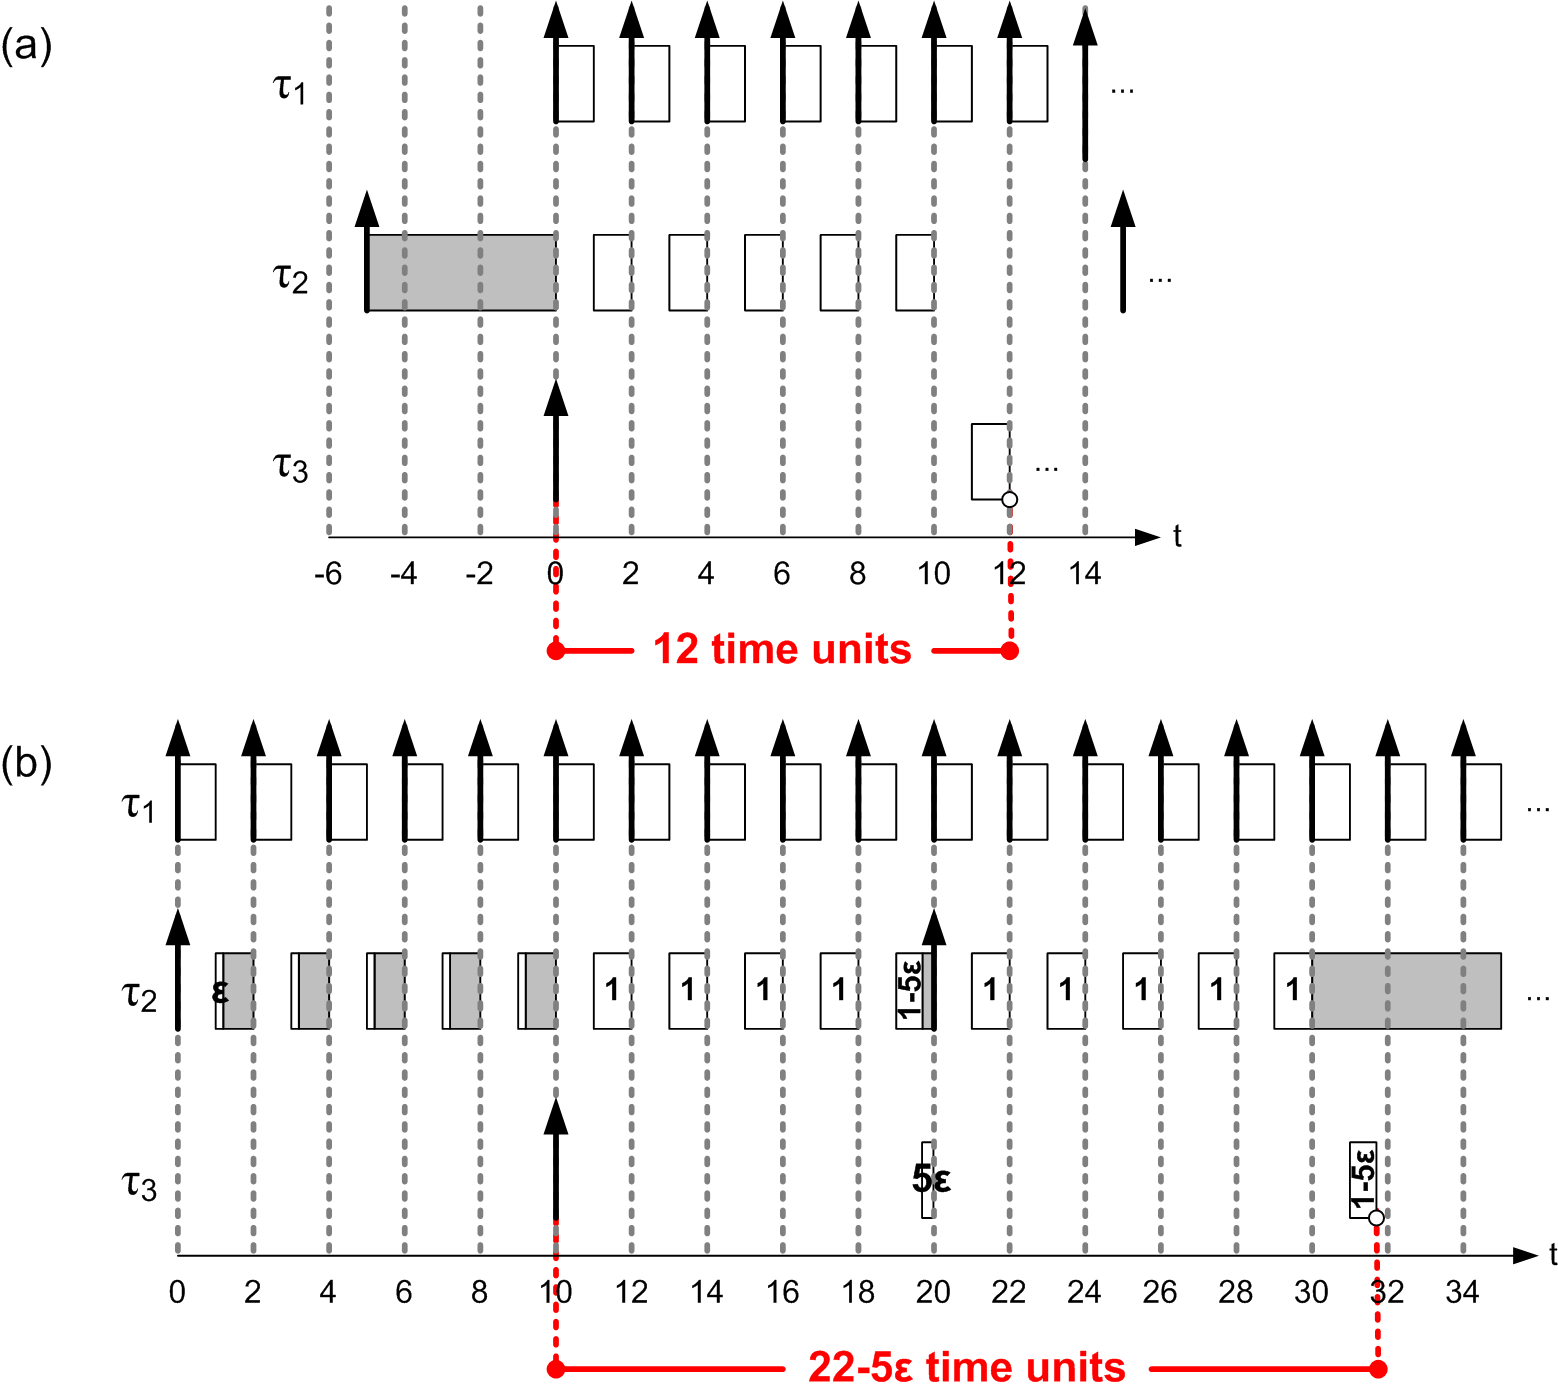
\includegraphics[width=\linewidth]{../figures/CounterexampleDynamicSuspension/counterexample_classic.png}
%\end{center}
%\caption{Two different schedules for the task set in Table~\ref{tab:counterexample-dynamic-suspension}.}
%\label{fig:counterexample-dynamic}
%\end{figure}

{\bf Consequences:} Since the results in \cite{ECRTS-AudsleyB04,RTAS-AudsleyB04,RTCSA-KimCPKH95,MingLiRTCSA1994} are fully based on the analysis in Eq.~(\ref{eq:dynamic-flawed}), the above unsafe example disproves the correctness of their analyses. The source of error comes from a wrong interpretation by Ming \cite{MingLiRTCSA1994} in 1994 with respect to a paper by Audsley et al. \cite{audsley-1993}.\footnote{The technical report of \cite{audsley-1993} is referred to in \cite{MingLiRTCSA1994}. Here we refer to the journal version.} Audsley et al. \cite{audsley-1993} explained that deferrable executions may result in arrival jitter and the jitter terms should be accounted while analyzing the worst-case response time. However, Ming \cite{MingLiRTCSA1994} interpreted that the jitter is the self-suspension time, which was not originally provided in \cite{audsley-1993}. Therefore, there was no proof of the correctness of the methods used in \cite{MingLiRTCSA1994}. The concept was adopted by Kim et al. \cite{RTCSA-KimCPKH95} in 1995. 

This misconception spread further when it was propagated by Lakshmanan et al.~\cite{lakshmanan-2009} in their derivation of worst-case response time bounds for
partitioned multiprocessor real-time locking protocols, which in turn was reused in several later works~\cite{zeng-2011,bbb-2013,yang-2013,kim-2014,han-2014,carminati-2014,yang-2014}. We explain the consequences and how to correct the later analyses in \mysectionref{}~\ref{sec:syn}. 
 
Moreover this counterexample also invalidates the comparison in \cite{RidouardR06}, which compares the schedulability tests from \cite{RTCSA-KimCPKH95} and \cite[Page 164-165]{Liu:2000:RS:518501}, since the result derived from \cite{RTCSA-KimCPKH95} is unsafe.

Independently, the authors of the results in \cite{ECRTS-AudsleyB04,RTAS-AudsleyB04} used the same methods in 2004 from different perspectives. A technical report that explains in greater detail how to correct this issue has been filed~\cite{BletsasReport2015}. 

{\bf Solutions:} It is explained and proved in \cite{huangpass:dac2015,BletsasReport2015} that the worst-case response time of task $\tau_k$ is bounded by the minimum $R_k$ with
\begin{equation}
R_k = C_k+ S_k+\sum_{\tau_i \in hp(k)}\ceiling{\frac{R_k+D_i-C_i}{T_i}} C_i,
\label{eq:dynamic-correct}
\end{equation}
for \emph{constrained-deadline} task systems under the assumption that every higher-priority task $\tau_i$ in $hp(k)$ can meet their relative deadline constraint. It is also safe to use $\ceiling{\frac{R_k+R_i-C_i}{T_i}}$ instead of $\ceiling{\frac{R_k+D_i-C_i}{T_i}}$ in the above equation if $R_i \leq D_i \leq T_i$.

\mysection{Incorrect Quantifications of Jitter (Segmented Self-Suspension)}
\label{sec:wrong-jitter-segmented}


We now explain a misconception in the literature regarding an
optimistic quantification of the jitter of segmented self-suspending
task systems under fixed-priority scheduling.

For the purpose of
bounding the interference from a segmented self-suspending task, the
analysis in~\cite{RTCSA-BletsasA05} reorders the computation segments
and the self-suspension intervals such that the computation segments
appear with decreasing execution times and the suspension intervals
appear with increasing suspension times. Upper-bounds are used for the
execution times of the former and lower-bounds for the lengths of the
latter. Among the self-suspension intervals, a ``notional''
self-suspension corresponding to the interval between the completion
of the task and its next arrival is included. The purpose of this
reordering step is to avoid having to consider different release
offsets for each interfering task (corresponding to its computational
segments). Using the following example of an implicit-deadline
segmented self-suspending task, with deterministic segment execution
times and self-suspension lengths, for convenience: Let $(C_i^1,
S_i^1, C_i^2, S_i^2, C_i^3)= (1,5,4,3,2)$ and $T_i=40$ and $R_i=25$.
The notional gap is $S_i^3=40-25=15$. After reordering, the parameters
become $(C_i^1, S_i^1, C_i^2, S_i^2, C_i^3, S_i^3) = (4,3,2,5,1,15)$.

%This is broadly analogous  to how Mok and Chen [REF] reorder task frames in their analysis for the multiframe task model.


% The second step, which was designed to capture the effects of the variation in the length of 
% computation segments or self-suspension intervals, will not be
% explained here as it does not have any effect if 
% there is no variation between the worst-case and the actual-case execution/suspension times.
% Each computation segment is modelled as a sporadic task with a fixed offset corresponding to the above
% rearrangement and a fixed jitter term to represent all computation segments of a given task.
% As reported in \cite{RTCSA-BletsasA05}, this jitter term corresponds to the maximum internal jitter, within the 
% activation of the task, of any computation segment, due to variability in the length of 
% preceding computation segments and self-suspension intervals.



In \cite{bletsas:thesis}, an error in the quantification of the
notional gap was already identified and fixed.  However, there remains
an error in the specified jitter term, designed to capture the variability in
the start times of the computation segments, relative to the job
release. In \cite{RTCSA-BletsasA05} it was incorrectly argued that it
is safe to only consider the variability in the lengths of
preceding computation segments and self-suspension intervals. In
the worst case though, one should also consider the variability resulting
from interference by tasks of even higher priorities.

Instead of going into the detailed mathematical formulations, we will demonstrate the misconception with the following example in Table~\ref{tab:counterexample-segmented}, which has only one self-suspending task $\tau_3$ and there is no variation between the worst-case and the actual-case execution/suspension times.
In
this specific example,  reordering has no effect. The
analysis in \cite{RTCSA-BletsasA05} can be imagined as replacing the
self-suspending task $\tau_3$ with a sporadic task without any jitter or self-suspension, with $C_3=2$ and $D_3=T_3=15$. Therefore, the analysis in \cite{RTCSA-BletsasA05}  concludes that the worst-case response time of task $\tau_4$ is at most $15$ since $C_4+\sum_{i=1}^{3}\ceiling{\frac{15}{T_i}} C_i = 3+ 6 + 4 + 2= 15$.


However, the perfectly legal schedule in Figure \ref{fig:counterexample-segmented} disproves this.
In that schedule, $\tau_1$, $\tau_2$, and $\tau_3$ arrive at $t=0$ and a job of $\tau_4$ arrives at $t=40$ and has a response time of 
$18$ time units.

\begin{table}[t]
\begin{center}
\begin{tabular}{|c||c|r|r|r|}
\hline
$\tau_i$ & $(C_i^1, S_i^1, C_i^2)$   &   $D_i$  &     $T_i$     \\ \hline
$\tau_1$ &  $(2, 0, 0)$                    &     $5$  &       $5$     \\ \hline
$\tau_2$ &  $(2, 0, 0)$                    &    $10$  &      $10$     \\ \hline
$\tau_3$ &  $(1, 5, 1)$            &    $15$  &      $15$     \\ \hline
$\tau_4$ &  $(3, 0, 0)$                   &    $?$  &   $\infty$    \\ \hline     
\end{tabular}
\end{center}
\caption{A set of segmented self-suspending tasks for demonstrating the misconception of the incorrect quantification of jitter in Section~\ref{sec:wrong-jitter-segmented}.}
\label{tab:counterexample-segmented}
\end{table}

\begin{figure}[t]
\centering
\def\uxfpga{0.25cm}
\scalebox{0.77}{
\begin{tikzpicture}[x=\uxfpga,y=\uy,auto, thick]
	\draw[->] (0,0) -- coordinate (xaxis) (62,0) node[anchor=north]{$t$};
	\foreach \x in {0,5,...,60}{
		\draw[-,below](\x,0) -- (\x,-0.3) node[] {\pgfmathtruncatemacro\yi{\x} \yi};
	}
	\foreach \x in {0,1,...,60}{
         \draw[-,very thin,lightgray, dashed](\x,0.3) -- (\x,8);
	}     
	\foreach \y in {2.03,4.03,6.03}{
		\draw[] (0,\y) -- (60,\y);
	}
       
	\begin{scope}[shift={(0,0)}]       
		\node[anchor=east] at (0, 0.5) {$\tau_4$};
		\draw[->] (40,0) -- (40,1.75);
		\draw[] (58.05,1) -- (58.05,1.5);
		\draw[dotted] (58.5,0.5) -- (60,0.5);
		\draw[<-,thin,red] (40,1.3) -- (48,1.3);
        	\draw[->,thin,red] (50,1.3) -- (58,1.3);
        	\node[anchor=east,red] at (50, 1.39) {18};
        	\node[task7, minimum width=2*\uxfpga, anchor=south west] at (48, 0){\footnotesize};         
        	\node[task7, minimum width=\uxfpga, anchor=south west] at (57, 0){\footnotesize};
	\end{scope}
      
    \begin{scope}[shift={(0,2)}]  
		\node[anchor=east] at (0, 0.5) {$\tau_3$};
		\foreach \x in {0,15,...,60}{
			\draw[<-](\x,1.75) -- (\x,0);
		}		
    		\draw[dotted] (60.5,0.5) -- (62,0.5);         
        	\node[task7, minimum width=\uxfpga, anchor=south west] at (4, 0){\footnotesize};
        	\foreach \y in {0.3,0.5,0.7}{ 
        		\draw[] (5,\y) -- (10,\y);
        	}
        	\draw[] (10,0) -- (10,1);
        	\node[task7, minimum width=\uxfpga, anchor=south west] at (14, 0){\footnotesize};
        	\node[task7, minimum width=\uxfpga, anchor=south west] at (17, 0){\footnotesize};
        	\foreach \y in {0.3,0.5,0.7}{ 
        	\draw[] (18,\y) -- (23,\y);}
        	\draw[] (23,0) -- (23,1);
        	\node[task7, minimum width=\uxfpga, anchor=south west] at (24, 0){\footnotesize};
        	\node[task7, minimum width=\uxfpga, anchor=south west] at (34, 0){\footnotesize};
        	\foreach \y in {0.3,0.5,0.7}{ 
        	\draw[] (35,\y) -- (40,\y);}
        	\draw[] (40,0) -- (40,1);
        	\node[task7, minimum width=\uxfpga, anchor=south west] at (44, 0){\footnotesize};
        	\node[task7, minimum width=\uxfpga, anchor=south west] at (47, 0){\footnotesize};
        	\foreach \y in {0.3,0.5,0.7}{ 
        		\draw[] (48,\y) -- (53,\y);
        	}
       	\draw[] (53,0) -- (53,1);
        	\node[task7, minimum width=\uxfpga, anchor=south west] at (54, 0){\footnotesize};
	\end{scope}
        
    \begin{scope}[shift={(0,4)}]        
		\node[anchor=east] at (0, 0.5) {$\tau_2$};
   		\foreach \x in {0,10,...,60}{
			\draw[<-](\x,1.75) -- (\x,0);
		}		
        	\draw[dotted] (60.5,0.5) -- (62,0.5);
        	\foreach \x in {2,12,...,52}{
			\node[task7, minimum width=2*\uxfpga, anchor=south west] at (\x, 0){\footnotesize};
		}
	\end{scope}

    \begin{scope}[shift={(0,6)}]        
		\node[anchor=east] at (0, 0.5) {$\tau_1$};
		\foreach \x in {0,5,...,55}{
			\draw[<-](\x,1.75) -- (\x,0);
			\node[task7, minimum width=2*\uxfpga, anchor=south west] at (\x, 0){\footnotesize};
		}
		\draw[<-](60,1.75) -- (60,0);		
		\draw[dotted] (60.5,0.5) -- (62,0.5);
	\end{scope}
\end{tikzpicture}}       
\caption{A schedule for demonstrating the misconception of the analysis in \cite{RTCSA-BletsasA05} by using the task set in Table  \ref{tab:counterexample-segmented}. }
\label{fig:counterexample-segmented}
\end{figure}

%\begin{figure}[t]
%\begin{center}
%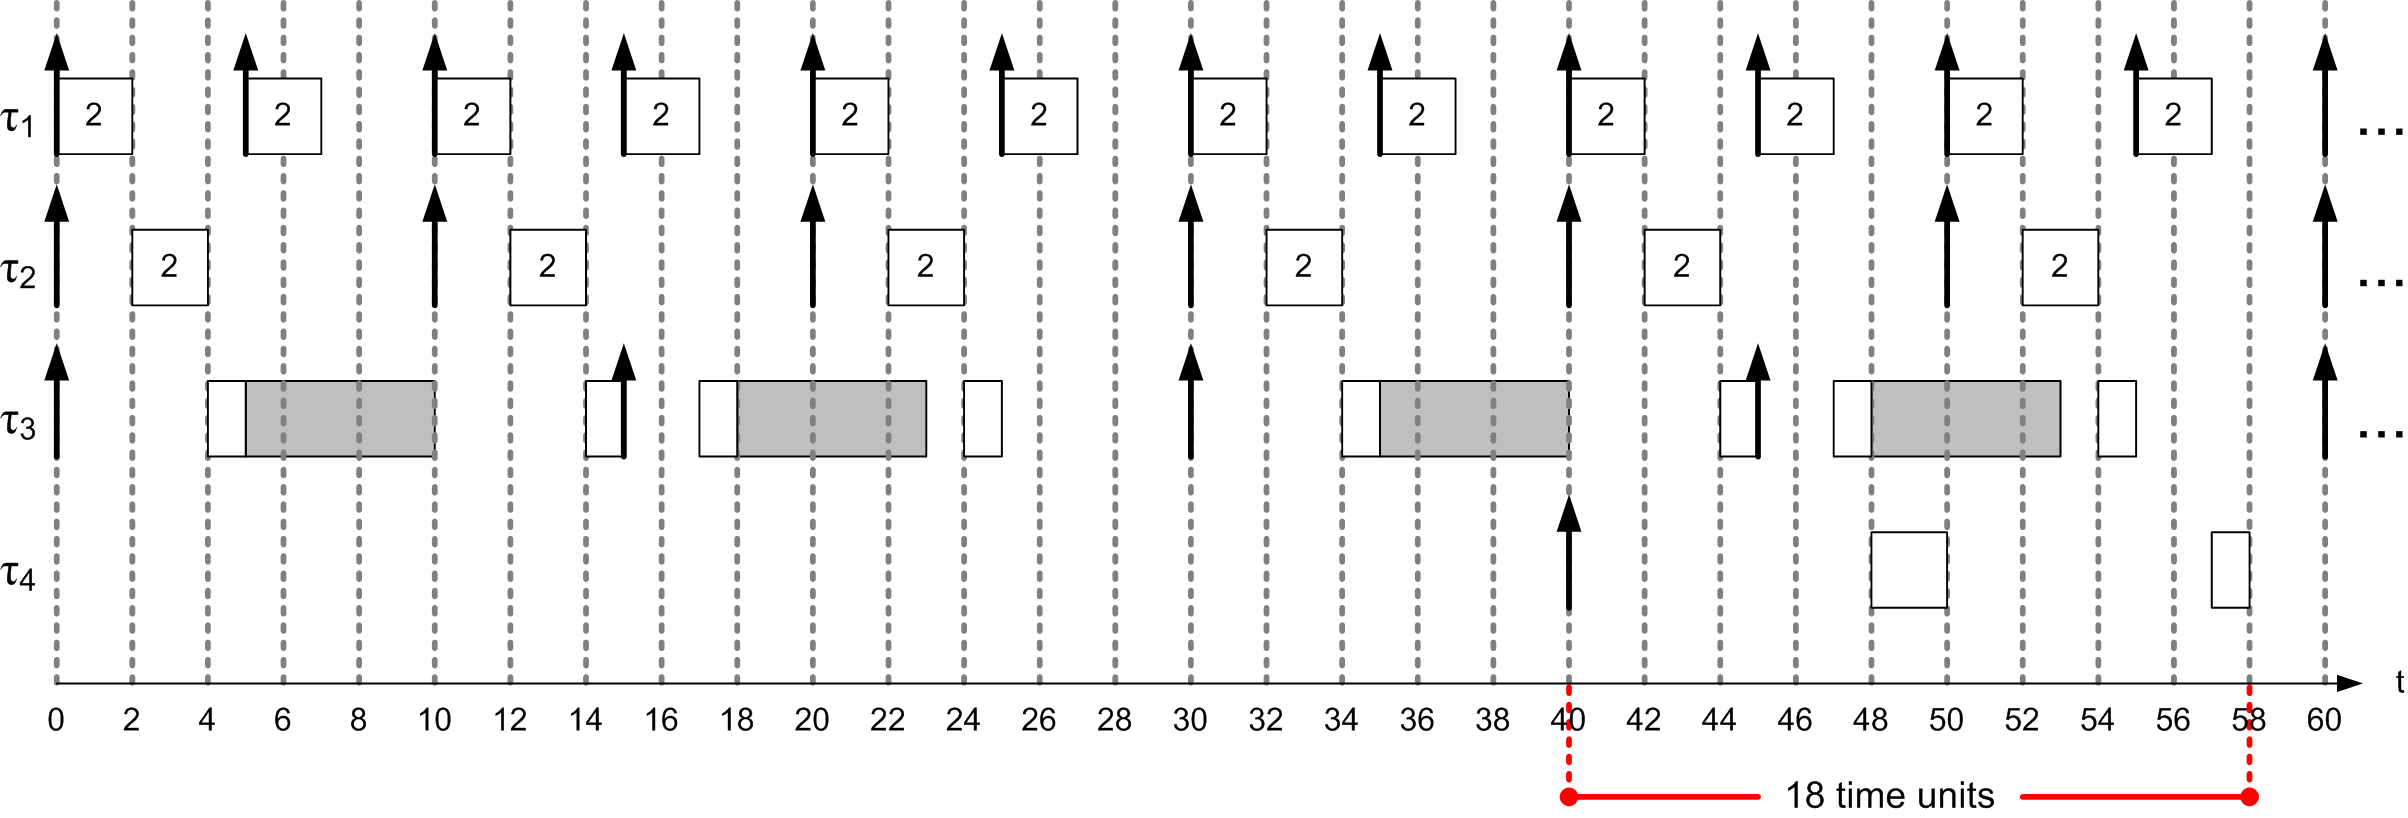
\includegraphics[width=\linewidth]{../figures/CounterexampleSegmentedSuspension/counterexample_synthetic.png}
%\end{center}
%\caption{A schedule for the task set in Table  \ref{tab:counterexample-segmented}. }
%\label{fig:counterexample-segmented}
%\end{figure}

{\bf Consequences:} This example shows that the analysis in \cite{RTCSA-BletsasA05} is flawed.  The authors in \cite{RTCSA-BletsasA05}  already filed a fix in~\cite{BletsasReport2015}.

{\bf Solutions:} When attempting to fix the error in the jitter quantification, there is no simple way to exploit the additional 
information provided by the segmented self-suspending task model.
However, quantifying the jitter of a self-suspending task $\tau_i$ with $D_i-C_i$ (or $R_i-C_i$) as in Section~\ref{sec:wrong-jitter-dynamic}  remains safe for constrained-deadline task systems since the dynamic self-suspension pattern is more general than a segmented self-suspension pattern.

\mysection{Incorrect Assumptions Regarding the Critical Instant}
\label{sec:wrong-critical}

Over the years, it has been well accepted that the characterization of the critical instant for self-suspending tasks is a complex problem. The complexity of verifying the existence of a feasible schedule for segmented self-suspending tasks has been proven to be ${\cal NP}$-hard in the strong sense \cite{Ridouard_2004}.  For segmented self-suspending tasks with constrained deadlines under fixed-priority scheduling, 
the complexity of verifying the schedulability of a task set has been left open until a recent proof of its co${\cal NP}$-hardness in the strong sense by Chen \cite{RTSS2016-suspension} and Mohaqeqi et al. \cite{DBLP:conf/rtns/MohaqeqiE016} in 2016 (see \mysectionref{}~\ref{sec:hardness}).

Before that, Lakshmanan and Rajkumar \cite{LR:rtas10} proposed a worst-case response time analysis for a one-segmented self-suspending task $\tau_k$ (with one self-suspension interval) with pseudo-polynomial time complexity assuming that 
\begin{itemize}
\item the scheduling algorithm is fixed-priority;
\item $\tau_k$ is the lowest-priority task;  and
\item all the higher-priority tasks are sporadic and non-self-suspending.
\end{itemize}
The analysis, presented in \cite{LR:rtas10}, is based on the notion of
a critical instant, \ie, an instant at which, considering the state of the system, an execution request for $\tau_k$ will generate the largest response time. This critical instant was defined as follows:
\begin{itemize}
	\item every task releases a job simultaneously with $\tau_k$;
	\item the jobs of higher-priority tasks that are eligible to be released during the self-suspension interval of $\tau_k$ are delayed to be aligned with the release of the subsequent computation segment of $\tau_k$; and
	\item all the remaining jobs of the higher-priority tasks are released with their minimum inter-arrival time.
\end{itemize}

This definition of the critical instant is similar to the definition of the critical instant of a non-self-suspending task. Specifically, it is based on the two intuitions that $\tau_k$ suffers the worst-case interference when (i) all higher-priority tasks release their first jobs simultaneously with $\tau_k$ and (ii) they all release as many jobs as possible in each computation segment of $\tau_k$. Although intuitively appealing, we provide examples showing that both statements are wrong. The examples provided below  first appeared in \cite{ecrts15nelissen}.

\mysubsection{A counterexample to the synchronous release}


\begin{figure}[t]
\centering
\def\uxfpga{0.4cm} 
\scalebox{1}{
	\begin{tikzpicture}[x=\uxfpga,y=\uy,auto, thick]
    \node[anchor=east] at (11.5, -1.75) {(a) Release jobs synchronously.};
    \node[anchor=east] at (28, -1.75) {(b) Do not release jobs synchronously.};
       
	\begin{scope}[shift={(0,0)}]       
    		\draw[->] (0,0) -- coordinate (xaxis) (12,0) node[anchor=north]{$t$};
    		\foreach \x in {0,2,...,10}{
			\draw[-,below](\x,0) -- (\x,-0.3) node[] {\pgfmathtruncatemacro\yi{\x} \yi};
		}
		\foreach \x in {0,1,...,10}{
        		\draw[-,very thin,lightgray, dashed](\x,0.3) -- (\x,6);
    		}
    		\foreach \y in {2.03,4.03}{
			\draw[] (0,\y) -- (10,\y);
		}		
		\node[anchor=east] at (0, 0.5) {$\tau_3$};
        \draw[->] (0,0) -- (0,1.75);
        \draw[dotted] (9.5,0.5) -- (10.3,0.5);
        \draw[<-,thin,red] (0,1.3) -- (3.9,1.3);
        \draw[->,thin,red] (5.1,1.3) -- (9,1.3);
        \draw[] (9.05,0) -- (9.05,1.5);
        \node[anchor=east,red] at (5, 1.39) {$9$}; 
        \node[task7, minimum width=\uxfpga, anchor=south west] at (2, 0){\footnotesize};     
        \node[task7, minimum width=3*\uxfpga, anchor=south west] at (6, 0){\footnotesize};    
		\foreach \y in {0.3,0.5,0.7}{        
			\draw[] (3,\y) -- (5,\y);
		}
		\draw[] (5,0) -- (5,1);
	\end{scope}
	
	\begin{scope}[shift={(0,2)}]       
		\node[anchor=east] at (0, 0.5) {$\tau_2$};
        \draw[->] (0,0) -- (0,1.75);
        \draw[dotted] (2.5,0.5) -- (3.3,0.5); 
        \node[task7, minimum width=\uxfpga, anchor=south west] at (1, 0){\footnotesize};
	\end{scope}	
        
    \begin{scope}[shift={(0,4)}]
    		\node[anchor=east] at (0, 0.5) {$\tau_1$};             
        \draw[->] (0,0) -- (0,1.75);
        \draw[dashed,->] (4,0) -- (4,1.75);
        \draw[->] (5,0) -- (5,1.75);
        \draw[->] (9,0) -- (9,1.75);
        \draw[dotted] (10.5,0.5) -- (11.3,0.5);
        \node[task7, minimum width=\uxfpga, anchor=south west] at (0, 0){\footnotesize};
        \node[task7, minimum width=\uxfpga, anchor=south west] at (5, 0){\footnotesize};
        \node[task7, minimum width=\uxfpga, anchor=south west] at (9, 0){\footnotesize};
	\end{scope}
	
	
	
	\begin{scope}[shift={(15,0)}]       
    		\draw[->] (0,0) -- coordinate (xaxis) (12,0) node[anchor=north]{$t$};
    		\foreach \x in {0,2,...,10}{
			\draw[-,below](\x,0) -- (\x,-0.3) node[] {\pgfmathtruncatemacro\yi{\x} \yi};
		}
		\foreach \x in {0,1,...,10}{
        		\draw[-,very thin,lightgray, dashed](\x,0.3) -- (\x,6);
    		}
    		\foreach \y in {2.03,4.03}{
			\draw[] (0,\y) -- (10,\y);
		}		
		\node[anchor=east] at (0, 0.5) {$\tau_3$};
        \draw[->] (0,0) -- (0,1.75);
        \draw[dotted] (10.5,0.5) -- (11.3,0.5); 
        \draw[<-,thin,red] (0,1.3) -- (4.3,1.3);
        \draw[->,thin,red] (5.7,1.3) -- (10,1.3);
        \draw[] (10.05,0) -- (10.05,1.5);
        \node[anchor=east,red] at (5.7, 1.39) {$10$}; 
        \node[task7, minimum width=\uxfpga, anchor=south west] at (1, 0){\footnotesize};     
        \node[task7, minimum width=2*\uxfpga, anchor=south west] at (6, 0){\footnotesize};
        \node[task7, minimum width=\uxfpga, anchor=south west] at (9, 0){\footnotesize};    
        \draw[] (4,0) -- (4,1);
		\foreach \y in {0.3,0.5,0.7}{        
			\draw[] (2,\y) -- (4,\y);
		}
	\end{scope}
	
	\begin{scope}[shift={(15,2)}]       
		\node[anchor=east] at (0, 0.5) {$\tau_2$};
        \draw[->] (4,0) -- (4,1.75);
        \draw[dotted] (6.5,0.5) -- (7.3,0.5); 
        \node[task7, minimum width=\uxfpga, anchor=south west] at (5, 0){\footnotesize};
	\end{scope}	
        
    \begin{scope}[shift={(15,4)}]             
        \node[anchor=east] at (0, 0.5) {$\tau_1$};
        \draw[dotted] (9.5,0.5) -- (10.3,0.5);
        \foreach \x in {0,4,8} {
			\draw[->] (\x,0) -- (\x,1.75);
			\node[task7, minimum width=\uxfpga, anchor=south west] at (\x, 0){\footnotesize};
        }
	\end{scope}	
\end{tikzpicture}}     
\caption{A counterexample to demonstrate the misconception of the synchronous release of all tasks in Section~\ref{sec:wrong-critical} based on the task set in Table~\ref{table:ex-synch-releases}.}
\label{fig:ex-synch-releases}
\end{figure}

\ifpaper
%\begin{figure}[t]
%  \centering
%\captionsetup[subfigure]{width=\columnwidth}
%  \subfloat[all tasks release a job synchronously.]{\label{fig:ex-phi} }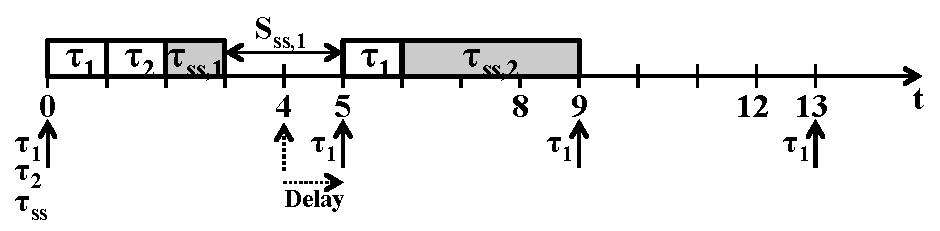
\includegraphics[width=0.85\linewidth]{../figures/ex-phi/ex-phi.pdf} \\
%  \subfloat[all tasks do not release a job synchronously.]{\label{fig:ex-no-phi} }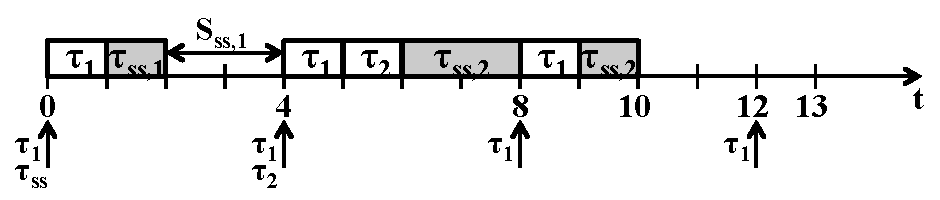
\includegraphics[width=0.85\linewidth]{../figures/ex-no-phi/ex-no-phi}
%  \caption{Counter-example to the synchronous release of all tasks (by \cite{LR:rtas10}).}
%  \label{fig:ex-synch-releases}
%\end{figure}
\fi

Consider three implicit deadline tasks with the parameters presented in Table~\ref{table:ex-synch-releases}. Let us assume that the priorities of the tasks are assigned using the rate monotonic policy (\ie, the smaller the period, the higher the priority). We are interested in computing the worst-case response time of $\tau_3$. Following the definition of the critical instant presented in \cite{LR:rtas10}, all three tasks must release a job synchronously at time $0$. Using the standard response-time analysis for non-self-suspending tasks, we get that the worst-case response time of the first computation segment of $\tau_3$ is equal to $R_3^1 = 3$. Because the second job of $\tau_1$ would be released in the self-suspension interval of $\tau_3$ if $\tau_1$ was strictly respecting its minimum inter-arrival time, the release of the second job of $\tau_1$ is delayed so as to coincide with the release of the second computation segment of $\tau_3$ (see Figure~\ref{fig:ex-synch-releases}(a)). Considering the fact that the second job of $\tau_2$ cannot be released before time instant $50$ and hence does not interfere with the execution of $\tau_3$, the response time of the second computation segment of $\tau_3$ is thus equal to $R_3^2=4$. In total, the worst-case response time of $\tau_3$ when all tasks release a job synchronously is equal to 
$$R_3 = R_3^1 + S_3^1 + R_3^2 = 3 + 2 +4 = 9.$$

\begin{table}[t] 
\centering
    \begin{tabular}{|c|c|c|}
 \hline
        & $(C_i^1, S_i^1, C_i^2)$ &  $D_i=T_i$\\ 
        \hline
        $\tau_1$ & (1, 0, 0) &  4\\ 
        $\tau_2$ &  (1, 0, 0) & 50  \\ 
        $\tau_3$ & (1, 2, 3) & 100  \\
        \hline
    \end{tabular} 
    \caption{A set of segmented self-suspending tasks for demonstrating the misconception
of the synchronous release of all tasks in Section~\ref{sec:wrong-critical}.}
    \label{table:ex-synch-releases}
\end{table}

Now, consider a job release pattern as shown in Figure~\ref{fig:ex-synch-releases}(b). Task $\tau_2$ does not release a job synchronously with task $\tau_3$ but with its second computation segment instead. The response time of the first computation segment of $\tau_3$ is thus reduced to $R_3^1=2$. However, both $\tau_1$ and $\tau_2$ can now release a job synchronously with the second computation segment of $\tau_3$, for which the response time is now equal to $R_3^2=6$ (see Figure~\ref{fig:ex-synch-releases}(b)). Thus, the total response time of $\tau_3$ in a scenario where not all higher-priority tasks release a job synchronously with $\tau_3$ is equal to 
$$R_3 = R_3^1 + S_3^1 + R_3^2 = 2+2+6 = 10.$$

{\bf Consequence:}  The synchronous release of all tasks does not necessarily generate the maximum interference for the self-suspending task $\tau_k$ and is thus not always a critical instant for $\tau_k$. 
It was however proven in \cite{ecrts15nelissen} that in the critical instant of a self-suspending task $\tau_k$, every higher-priority task releases a job synchronously with the arrival of at least one computation segment of $\tau_k$, but not all higher-priority tasks must release a job synchronously with the same computation segment.

\mysubsection{A counterexample to the minimum inter-release time}

Consider a task set of $4$ tasks $\tau_1, \tau_2, \tau_3, \tau_4$ in which $\tau_1$, $\tau_2$ and $\tau_3$ are non-self-suspending sporadic tasks and $\tau_4$ is a self-suspending task with the lowest priority. The tasks have the parameters provided in Table~\ref{table:ex-num-releases}. The worst-case response time of $\tau_4$ is obtained when $\tau_1$ releases a job synchronously with the second computation segment of $\tau_4$ while $\tau_2$ and $\tau_3$ must release a job synchronously with the first computation segment of $\tau_4$.

\begin{table}[t]
\centering
    \begin{tabular}{|c|c|c|}
 \hline
        & $(C_i^1, S_i^2, C_i^2)$ &  $D_i=T_i$\\ 
        \hline
        $\tau_1$ & (4, 0, 0) &  8\\ 
        $\tau_2$ &  (1, 0, 0) & 10 \\ 
        $\tau_3$ & (1, 0, 0) & 17 \\
        $\tau_4$ & (265, 2, 6) & 1000\\
        \hline
    \end{tabular} 
    \caption{A set of segmented self-suspending tasks used to  demonstrate that it is a misconception to believe that releasing interfering jobs as early and often as possible yields a worst-case scenario, as discussed in Section~\ref{sec:wrong-critical}. }
    \label{table:ex-num-releases}
\end{table}

Consider two scenarios with respect to the job release pattern. Scenario~1 is a result of the proposed critical instant, in which the jobs of the higher-priority non-self-suspending tasks are released as early and often as possible to interfere with each computation segment of $\tau_4$. 
 In Scenario~2, one less job of task $\tau_1$ is released before the first computation segment of the self-suspending task finishes.
We show that the WCRT of $\tau_4$  is higher in the second scenario.

Scenario~1 is depicted in Fig.~\ref{fig:ex_crit_inst2}(a), and Scenario~2 in Fig.~\ref{fig:ex_crit_inst2}(b). The first $765$ time units are omitted in both figures. In both scenarios, the schedules of the jobs are identical in this initial time window.  
The first jobs of $\tau_1$, $\tau_2$, and $\tau_3$ are released synchronously with the arrival of the first computation segment of $\tau_4$ at time $0$. The subsequent jobs of these three tasks are released as early and often as possible respecting the minimum inter-arrival times of the respective tasks. That is, they are released periodically with periods $T_1$, $T_2$ and $T_3$, respectively. With this release pattern, it is easy to compute that the $97^\text{th}$ job of $\tau_1$ is released at time $768$, the $78^\text{th}$ job of $\tau_2$ at time $770$ and the $46^\text{th}$ job of $\tau_3$ at time $765$. As a consequence, at time $765$, $\tau_4$ has finished executing $259$ time units of its first execution segment out of $265$ in both scenarios, \ie, $765 - 96 \times 4 - 77 \times 1 - 45 \times 1 = 259$.  From time $765$ onward, we separately consider Scenarios~1 and~2.
%\begin{figure}
%  \centering
%  \subfloat[Scenario 1. Jobs are released as often as possible.]{\label{fig:ex_crit_inst2sc1} 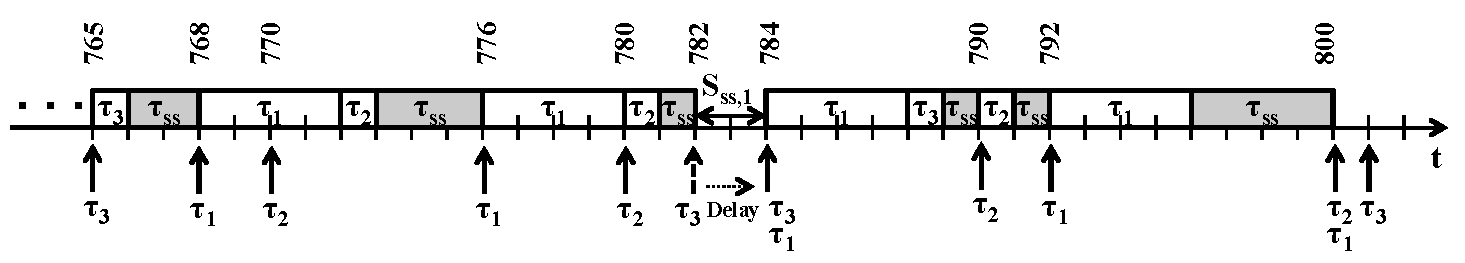
\includegraphics[height=1.95cm, width=\linewidth]{../figures/ex2sc1}} \\
%  \subfloat[Scenario 2. Jobs are not released as often as possible.]{\label{fig:ex_crit_inst2sc2} %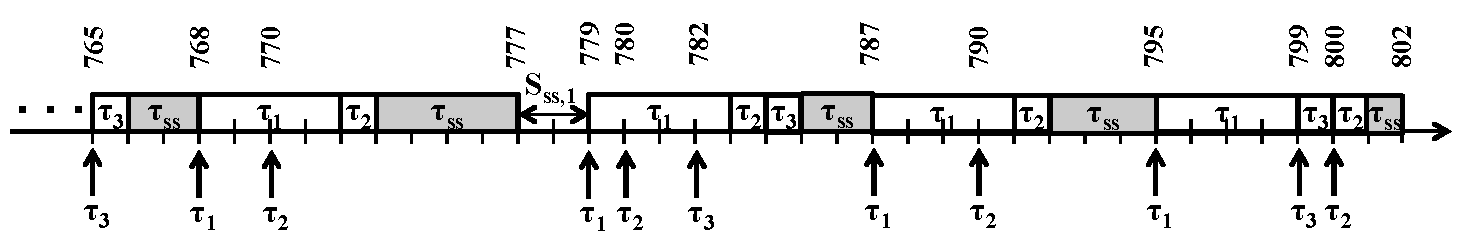
\includegraphics[height=1.8cm, width=\linewidth]{../figures/ex2sc2}}
%  \caption{Example showing that releasing higher priority jobs as often as possible may not always cause the maximum interference on a self-suspending task.}
%  \label{fig:ex_crit_inst2}
%\end{figure}

\begin{figure}[t]
\centering
\def\uxfpga{0.4cm} 
\subfloat[Scenario 1. Jobs are released as early and often as possible to interfere with each computation segment of task $\tau_k$.]{
\scalebox{0.73}{
	\begin{tikzpicture}[x=\uxfpga,y=\uy,auto, thick]
    \draw[->] (0,0) -- coordinate (xaxis) (39,0) node[anchor=north]{$t$};
    \foreach \x in {0,5,...,35}{
		\draw[-,below](\x,0) -- (\x,-0.3) node[] {\pgfmathtruncatemacro\yi{\x+765} \yi};
	}
	\foreach \x in {0,1,...,38}{
         \draw[-,very thin,lightgray, dashed](\x,0) -- (\x,8);
	}	
	\foreach \y in {2.03,4.03,6.03}{
		\draw[] (0,\y) -- (38,\y);
	}
	
	\begin{scope}[shift={(0,0)}]
		\node[anchor=east] at (0, 0.5) {$\tau_4$};
        \node[task7, minimum width=2*\uxfpga, anchor=south west] at (1, 0){\footnotesize};
        \node[task7, minimum width=3*\uxfpga, anchor=south west] at (8, 0){\footnotesize};
        \node[task7, minimum width=\uxfpga, anchor=south west] at (16, 0){\footnotesize};
        \node[task7, minimum width=\uxfpga, anchor=south west] at (24, 0){\footnotesize};
        \node[task7, minimum width=\uxfpga, anchor=south west] at (26, 0){\footnotesize};
        \node[task7, minimum width=4*\uxfpga, anchor=south west] at (31, 0){\footnotesize};  
    		\foreach \y in {0.3,0.5,0.7}{ 
    			\draw[] (17,\y) -- (19,\y);
        	} 
        \draw[] (19,0) -- (19,1);
	\end{scope}

	\begin{scope}[shift={(0,2)}]
		\node[anchor=east] at (0, 0.5) {$\tau_3$};
        \draw[->] (0,0) -- (0,1.75);
        \draw[->] (19,0) -- (19,1.75);
        \draw[->] (36,0) -- (36,1.75);
        \draw[->, dashed] (17,0) -- (17,1.75);
        \draw[<->, thin, red] (17,0.5)--(19,0.5);
        \node[anchor=east,red] at (19.3, 1) {Delay}; 
    		\node[task7, minimum width=\uxfpga, anchor=south west] at (0, 0){\footnotesize};
    		\node[task7, minimum width=\uxfpga, anchor=south west] at (23, 0){\footnotesize};
	\end{scope}

	\begin{scope}[shift={(0,4)}]
		\node[anchor=east] at (0, 0.5) {$\tau_2$};
        \foreach \x in {5,15,...,35}{ 
			\draw[->] (\x,0) -- (\x,1.75);            		
        	}
        	\node[task7, minimum width=\uxfpga, anchor=south west] at (7, 0){\footnotesize};
        	\node[task7, minimum width=\uxfpga, anchor=south west] at (15, 0){\footnotesize};
        	\node[task7, minimum width=\uxfpga, anchor=south west] at (25, 0){\footnotesize};
	\end{scope}                

	\begin{scope}[shift={(0,6)}]
		\node[anchor=east] at (0, 0.5) {$\tau_1$};
        \foreach \x in {3,11,...,27}{ 
			\draw[->] (\x,0) -- (\x,1.75);     
			\node[task7, minimum width=4*\uxfpga, anchor=south west] at (\x, 0){\footnotesize};       		
        	}
        	\draw[->] (35,0) -- (35,1.75);
	\end{scope}                
	
\end{tikzpicture}} }

\subfloat[Scenario 2. Jobs are not released as early and often as possible.]{
\scalebox{0.73}{
	\begin{tikzpicture}[x=\uxfpga,y=\uy,auto, thick]
    \draw[->] (0,0) -- coordinate (xaxis) (39,0) node[anchor=north]{$t$};
    \foreach \x in {0,5,...,35}{
		\draw[-,below](\x,0) -- (\x,-0.3) node[] {\pgfmathtruncatemacro\yi{\x+765} \yi};
	}
	\foreach \x in {0,1,...,38}{
         \draw[-,very thin,lightgray, dashed](\x,0) -- (\x,8);
	}	
	\foreach \y in {2.03,4.03,6.03}{
		\draw[] (0,\y) -- (38,\y);
	}
	
	\begin{scope}[shift={(0,0)}]
		\node[anchor=east] at (0, 0.5) {$\tau_4$};
        \node[task7, minimum width=2*\uxfpga, anchor=south west] at (1, 0){\footnotesize};
        \node[task7, minimum width=4*\uxfpga, anchor=south west] at (8, 0){\footnotesize};
        \node[task7, minimum width=2*\uxfpga, anchor=south west] at (20, 0){\footnotesize};
        \node[task7, minimum width=3*\uxfpga, anchor=south west] at (27, 0){\footnotesize};
        \node[task7, minimum width=\uxfpga, anchor=south west] at (36, 0){\footnotesize};
    		\foreach \y in {0.3,0.5,0.7}{ 
    			\draw[] (12,\y) -- (14,\y);
        	} 
        \draw[] (14,0) -- (14,1);
	\end{scope}

	\begin{scope}[shift={(0,2)}]
		\node[anchor=east] at (0, 0.5) {$\tau_3$};
        \draw[->] (0,0) -- (0,1.75);
        \draw[->] (17,0) -- (17,1.75);
        \draw[->] (34,0) -- (34,1.75);
    		\node[task7, minimum width=\uxfpga, anchor=south west] at (0, 0){\footnotesize};
    		\node[task7, minimum width=\uxfpga, anchor=south west] at (19, 0){\footnotesize};
    		\node[task7, minimum width=\uxfpga, anchor=south west] at (34, 0){\footnotesize};
	\end{scope}

	\begin{scope}[shift={(0,4)}]
		\node[anchor=east] at (0, 0.5) {$\tau_2$};
        \foreach \x in {5,15,...,35}{ 
			\draw[->] (\x,0) -- (\x,1.75);            		
        	}
        	\node[task7, minimum width=\uxfpga, anchor=south west] at (7, 0){\footnotesize};
        	\node[task7, minimum width=\uxfpga, anchor=south west] at (18, 0){\footnotesize};
        	\node[task7, minimum width=\uxfpga, anchor=south west] at (26, 0){\footnotesize};
        	\node[task7, minimum width=\uxfpga, anchor=south west] at (35, 0){\footnotesize};
	\end{scope}                

	\begin{scope}[shift={(0,6)}]
		\node[anchor=east] at (0, 0.5) {$\tau_1$};
        \foreach \x in {3,14,22,30}{ 
			\draw[->] (\x,0) -- (\x,1.75);     
			\node[task7, minimum width=4*\uxfpga, anchor=south west] at (\x, 0){\footnotesize};       		
        	}
        	\draw[->] (38,0) -- (38,1.75);
        \draw[->, dashed] (11,0) -- (11,1.75);
        \draw[<->, thin, red] (11,0.5)--(14,0.5);
        \node[anchor=east,red] at (13.8, 1) {Delay}; 

	\end{scope}                
\end{tikzpicture}} }
\caption{An example based on the task set in Table~\ref{table:ex-num-releases} showing that releasing higher-priority jobs as early and often as possible to interfere with each computation segment of task $\tau_k$ may not always cause the maximum interference on a self-suspending task.}
\label{fig:ex_crit_inst2}
\end{figure}

\noindent\textbf{Scenario 1.} Continuing the release of jobs of the non-self-suspending tasks as early and often as possible without violating their minimum inter-arrival times, the first computation segment of $\tau_4$ finishes its execution at time $782$ as shown in Fig.~\ref{fig:ex_crit_inst2}(a). After completion of its first computation segment, $\tau_4$ self-suspends for two time units until time $784$. As $\tau_3$ would have released a job within the self-suspension interval, we delay the release of that job from time $782$ to $784$ in order to maximize the interference exerted by $\tau_3$ on the second computation segment of $\tau_4$ as shown in Fig.~\ref{fig:ex_crit_inst2}(a). Note that, in order to respect its minimum inter-arrival time, $\tau_2$ has an offset of $6$ time units with the arrival of the second computation segment of $\tau_4$. Upon following the rest of the schedule, it can easily be seen that the job of $\tau_4$ finishes its execution at time $800$.

\noindent\textbf{Scenario 2.} As shown in Fig.~\ref{fig:ex_crit_inst2}(b), the release of a job of task $\tau_1$ is skipped at time $776$ in comparison to Scenario~1. As a result, the execution of the first computation segment of $\tau_4$ is completed at time $777$, thereby causing one job of $\tau_2$ that was released at time $780$ in Scenario 1, to \emph{not} be released during the execution of the first computation segment of $\tau_4$. The response time of the first computation segment of $\tau_4$ is thus reduced by $C_1 + C_2 = 5$ time units in comparison to Scenario 1 (see Fig.~\ref{fig:ex_crit_inst2}(a)). Note that this deviation from Scenario 1 does not affect the fact that $\tau_1$ still releases a job synchronously with the second computation segment of $\tau_4$. The next job of $\tau_3$ however, is not released in the suspension interval anymore but $3$ time units after the arrival of $\tau_4$'s second computation segment. Moreover, the offset of $\tau_2$ with respect to the start of the second computation segment is reduced by $C_1 + C_2 = 5$ time units. This causes an extra job of $\tau_2$ to be released in the second computation segment of $\tau_4$, initiating a cascade effect: an extra job of $\tau_1$ is released in the second computation segment at time $795$, which in turn causes the release of an extra job of $\tau_3$, itself causing the arrival of one more job of $\tau_2$. Consequently, the response time of the second computation segment increases by $C_2 + C_1 + C_3 + C_2 = 7$ time units. Overall, the response time of $\tau_4$ increases by $7 - 5 = 2$ time units in comparison to Scenario~1. This is reflected in Figure~\ref{fig:ex_crit_inst2}(b) as the job of $\tau_4$ finishes its execution at time $802$.\\


{\bf Consequence:} This counterexample proves that the response time of a self-suspending task $\tau_k$ can be larger when the tasks in $hp(k)$ do not release jobs as early and often as possible to interfere with each computation segment of task $\tau_k$.

{\bf Solution:} The problem of defining the critical instant remains open even for the special case where only the lowest-priority task is self-suspending. Nelissen et al. propose a limited solution in \cite{ecrts15nelissen} based on an exhaustive search with exponential time complexity.

\mysection{Counting Highest-Priority Self-Suspension Time to Reduce the Interference}
\label{sec:wrong-highest-priority}

We now present a misconception which exploits the  self-suspension time  of the highest-priority task to reduce its interference to the lower-priority sporadic tasks. 
We consider fixed-priority preemptive scheduling for $n$ self-suspending sporadic real-time tasks on a single processor, in which $\tau_1$ is the highest-priority task and $\tau_n$ is the lowest-priority task.
% We focus on constrained-deadline task systems with $D_i \leq T_i$ or implicit-deadline systems with $D_i=T_i$ for $i=1,\ldots,n$.
Let us consider the simplest setting of such a case:
\begin{itemize}
\item there is only one self-suspending task with the highest priority, \ie, $\tau_1$,
\item the self-suspension time is fixed, \ie, early return of self-suspension has to be controlled by the scheduler, and
\item the actual execution time of the self-suspending task is always equal to its worst-case execution time.
\end{itemize}
Denote this task set as $\Gamma_{1s}$ (as also used in \cite{RTSS-KimANR13}).  Since $\tau_1$ is the highest-priority task, its execution behavior is static under the above assumptions. The misconception here is to identify the critical instant  (Theorem 2 in \cite{RTSS-KimANR13}) as follows: ``a critical instant occurs when all the tasks are released at the same time if $C_1 +S_1 < C_i  \leq T_1-C_1-S_1 \mbox{ for } i \in\{i|i\in Z^{+} \mbox{ and } 1<i\leq n\}$ is satisfied.'' This observation leads to a wrong implication that causes the self-suspension time (if it is long enough) to \emph{reduce} the computation demand of $\tau_i$ for interfering with lower-priority tasks. 


\begin{table} [t]
\centering
    \begin{tabular}{|c|c|c|}
 \hline
        & $(C_i^1, S_i^1, C_i^2)$ &  $D_i=T_i$\\ 
        \hline
        $\tau_1$ & $(\epsilon, 1, 1)$ &  $4+10\epsilon$\\ 
        $\tau_2$ &  ($2+2\epsilon$, 0, 0) & 6  \\ 
        $\tau_3$ & ($2+2\epsilon$, 0, 0) & 6  \\
        \hline
    \end{tabular} 
    \caption{A set of segmented self-suspending tasks for demonstrating the misconception
to reduce the interference by exploiting the highest-priority self-suspension time in Section~\ref{sec:wrong-highest-priority}, where $0 < \epsilon \leq 0.1$.}
    \label{table:ex-highest-priority}
\end{table}


{\it Counterexample to Theorem 2 in \cite{RTSS-KimANR13}:} Let $\epsilon$ be a positive and very small number, \ie, $0 < \epsilon \leq 0.1$.  Consider the three tasks listed in Table~\ref{table:ex-highest-priority}. By the setting, $2+\epsilon = C_1+S_1 < C_i = 2+2\epsilon \leq T_1-C_1-S_1 = 2+9\epsilon$ for $i=2,3$. The above claim states that the worst case is to release all the three tasks together at time $0$ (as shown in Figure~\ref{fig:counterexample-reduce-interf}(a)). The analysis shows that the response time of task $\tau_3$ is at most $5+6\epsilon$. However, if we release task $\tau_1$ at time $0$ and release task $\tau_2$ and task $\tau_3$ at time $1+\epsilon$ (as shown in Figure~\ref{fig:counterexample-reduce-interf}(b)), the response time of the first job of task $\tau_3$ is $6+5\epsilon$. 

\begin{figure}[t]
\centering
\def\uxfpga{0.4cm} 
\scalebox{1}{
	\begin{tikzpicture}[x=\uxfpga,y=\uy,auto, thick]
    \node[anchor=east] at (11.5, -1.75) {(a) Release jobs synchronously.};
    \node[anchor=east] at (28, -1.75) {(b) Do not release jobs synchronously.};
       
	\begin{scope}[shift={(0,0)}]       
    		\draw[->] (0,0) -- coordinate (xaxis) (12,0) node[anchor=north]{$t$};
	    \foreach \x in {0,2,...,10}{
			\draw[-,below](\x,0) -- (\x,-0.3) node[] {\pgfmathtruncatemacro\yi{\x} \yi};
		}
		\foreach \x in {0,1,...,10}{
        		\draw[-,very thin,lightgray, dashed](\x,0.3) -- (\x,6);
    		}
    		\foreach \y in {2.03,4.03}{
			\draw[] (0,\y) -- (10,\y);
		}
		\node[anchor=east] at (0, 0.5) {$\tau_3$};
        \draw[->] (0,0) -- (0,1.75);
        \draw[->] (6,0) -- (6,1.75);       
        \draw[dotted] (6.5,0.5) -- (7.3,0.5);
        \draw[<-,thin,red] (0,1.3) -- (1.5,1.3);
        \draw[->,thin,red] (4.1,1.3) -- (5.6,1.3);
        \node[anchor=east,red] at (4.2, 1.39) {$5+6\varepsilon$};         
        \draw[] (3.3,1.03) -- (4.8,1.03);
        \draw[] (3.3,0) -- (3.3,1);
        \draw[] (4.8,0) -- (4.8,1);
        \draw[] (5,1.03) -- (5.6,1.03);
        \draw[] (5,0) -- (5,1);
        \draw[] (5.6,0) -- (5.6,1.5);
	\end{scope}
	
	\begin{scope}[shift={(0,2)}]       
        \node[anchor=east] at (0, 0.5) {$\tau_2$};
        \draw[->] (0,0) -- (0,1.75);
        \draw[->] (6,0) -- (6,1.75);
        \draw[dotted] (6.5,0.5) -- (7.3,0.5); 
        \node[task7, minimum width=\uxfpga, anchor=south west] at (0.2, 0){\footnotesize};
        \draw[] (2.2,0.03) -- (3.3,0.03);
        \draw[] (2.2,1.03) -- (3.3,1.03);
        \draw[] (2.2,0.03) -- (2.2,1.03);
        \draw[] (3.3,0.03) -- (3.3,1.03);
	\end{scope}	
        
    \begin{scope}[shift={(0,4)}]
    		\node[anchor=east] at (0, 0.5) {$\tau_1$};
    		\draw[dotted] (10.1,0.5) -- (11,0.5);    		
    		\foreach \x in {0,4.8}{
    			\draw[->] (\x,0) -- (\x,1.75);
    			\node[task7, minimum width=\uxfpga, anchor=south west] at (\x+1.2, 0){\footnotesize};
    			\draw[] (\x,1.03) -- (\x+0.2,1.03);
    			\draw[] (\x,0.03) -- (\x+0.2,0.03);
    			\draw[] (\x+0.2,0) -- (\x+0.2,1);
    			\foreach \y in {0.3,0.5,0.7}{
    			\draw[] (\x+0.2,\y) -- (\x+1.2,\y);
    		}}
    		\draw[->] (9.6,0) -- (9.6,1.75);
	\end{scope}
	
	
	
	
	\begin{scope}[shift={(15,0)}]       
    		\draw[->] (0,0) -- coordinate (xaxis) (12,0) node[anchor=north]{$t$};
	    \foreach \x in {0,2,...,10}{
			\draw[-,below](\x,0) -- (\x,-0.3) node[] {\pgfmathtruncatemacro\yi{\x} \yi};
		}
		\foreach \x in {0,1,...,10}{
        		\draw[-,very thin,lightgray, dashed](\x,0.3) -- (\x,6);
    		}
    		\foreach \y in {2.03,4.03}{
			\draw[] (0,\y) -- (10,\y);
		}
        \node[anchor=east] at (0, 0.5) {$\tau_3$};
        \draw[->] (1.2,0) -- (1.2,1.75);
        \draw[<-,red] (7.2,0) -- (8.6,1.3);
        \node[anchor=east,red] at (10.5, 1.68) {miss};
        \draw[<-,thin,red] (1.2,1.3) -- (3,1.3);
        \draw[->,thin,red] (5.7,1.3) -- (7.6,1.3);
        \node[anchor=east,red] at (5.8, 1.4) {$6+5\varepsilon$};
        \draw[] (4.25,1.03) -- (4.8,1.03);
        \draw[] (4.25,0.03) -- (4.8,0.03);
        \draw[] (4.25,0.03) -- (4.25,1.03);
        \draw[] (4.8,0.03) -- (4.8,1.03);
        \node[task7, minimum width=\uxfpga, anchor=south west] at (5, 0){\footnotesize};
        \draw[] (7,1.03) -- (7.6,1.03);
        \draw[] (7,0.03) -- (7,1.03);
        \draw[] (7.6,0.03) -- (7.6,1.5);
	\end{scope}
	
	\begin{scope}[shift={(15,2)}]       
		\node[anchor=east] at (0, 0.5) {$\tau_2$};
        \draw[->] (1.2,0) -- (1.2,1.75);
        \draw[->] (7.2,0) -- (7.2,1.75);
        \draw[] (2.2,1.03) -- (4.25,1.03);
        \draw[] (2.2,0.03) -- (4.25,0.03);
        \draw[] (2.2,0.03) -- (2.2,1.03);
        \draw[] (4.25,0.03) -- (4.25,1.03);
	\end{scope}	
        
    \begin{scope}[shift={(15,4)}]             
    		\node[anchor=east] at (0, 0.5) {$\tau_1$};
    		\foreach \x in {0,4.8}{
    			\draw[->] (\x,0) -- (\x,1.75);
    			\node[task7, minimum width=\uxfpga, anchor=south west] at (\x+1.2, 0){\footnotesize};
    			\draw[] (\x,1.03) -- (\x+0.2,1.03);
    			\draw[] (\x,0.03) -- (\x+0.2,0.03);
    			\draw[] (\x+0.2,0) -- (\x+0.2,1);
    			\foreach \y in {0.3,0.5,0.7}{
    			\draw[] (\x+0.2,\y) -- (\x+1.2,\y);
    		}}
    		\draw[->] (9.6,0) -- (9.6,1.75);
	\end{scope}	
 \end{tikzpicture}}     
  \caption{A counterexample presented in Section~\ref{sec:wrong-highest-priority} for demonstrating the misconception on the synchronous release used in Theorem 2 in \cite{RTSS-KimANR13}, based on the task set in Table~\ref{table:ex-highest-priority}.}
  \label{fig:counterexample-reduce-interf}
\end{figure}

This misconception also leads to a wrong statement in Theorem 3 in \cite{RTSS-KimANR13}:
\begin{quote}
{\it Theorem 3 in \cite{RTSS-KimANR13}}: For a taskset $\Gamma_{1s}$ with implicit deadlines, $\Gamma_{1s}$ is schedulable if the total utilization of the taskset is less than or equal to $n((2+2\gamma)^{\frac{1}{n}}-1)-\gamma$, where $n$ is the number of tasks in $\Gamma_{1s}$, and $\gamma$ is the ratio of
$S_1$ to $T_1$ and lies in the range of $0$ to $2^{\frac{1}{n-1}}-1$. 
\end{quote}


{\it Counterexample of Theorem 3 in \cite{RTSS-KimANR13}:} Suppose that the self-suspending task $\tau_1$ has two computation segments, with $C_1^1 = C_1-\epsilon$, $C_1^2 = \epsilon$, and $S_1=S_1^1 > 0$ with very small $0 < \epsilon \ll C_1^1$. For such an example, it is obvious that this self-suspending highest-priority task is like an ordinary sporadic task, \ie, self-suspension does not matter. 
 In this counterexample, the utilization bound is still Liu and Layland bound $n(2^{\frac{1}{n}}-1)$ \cite{Liu_1973}, regardless of the ratio of $S_1/T_1$. 

The source of the error of Theorem 3 in \cite{RTSS-KimANR13} is due to its Theorem 2 and the footnote 4 in \cite{RTSS-KimANR13}, which claims that the case in Figure 7 in \cite{RTSS-KimANR13} is the worst case. This statement is incorrect and can be disproved with the above counterexample. 


{\bf Consequences:} Theorems 2 and 3 in \cite{RTSS-KimANR13} are flawed.  

{\bf Solutions:} The three assumptions, \ie, one highest-priority segmented self-suspending task, controlled suspension behavior, and controlled execution time  in \cite{RTSS-KimANR13} actually imply that the self-suspending behavior of task $\tau_1$ can be modeled as several sporadic tasks with the same minimum inter-arrival time. More precisely, there is no need to consider self-suspension of task $\tau_1$, but we have to effectively consider each computation segment as a highest-priority sporadic task during the response time analysis. When the $j$-th computation segment of task $\tau_1$ starts its execution at time $t$, the earliest time for this computation segment to be executed again in the next job of task $\tau_1$ is at least $t+T_1$. 

Therefore, a constrained-deadline task $\tau_k$ can be feasibly scheduled by the fixed-priority scheduling strategy if $C_1+S_1 \leq D_1$ and for $2 \leq k \leq n$
  \begin{equation}
    \label{eq:tda-fixed}
\exists 0 < t \leq D_k, \qquad C_k + \sum_{i=1}^{k-1}\ceiling{\frac{t}{T_i}}C_i \leq t.    
  \end{equation}
%This also implies that the utilization bound (for implicit-deadline task systems) is still Liu and Layland bound $n(2^{\frac{1}{n}}-1)$ \cite{Liu_1973}, regardless of the ratio of $S_1/T_1$. 

A version of~\cite{RTSS-KimANR13} correcting the problems mentioned in this section can be found in~\cite{Kim2016}.

\mysection{Incorrect Analysis of Segmented Fixed-Priority Scheduling with Periodic Enforcement}
\label{sec:wrong-periodic}

We now introduce misconceptions that may happen due to periodic enforcement if it is not carefully adopted for segmented self-suspending task systems. As mentioned in Section~\ref{sec:static-period-enforce}, we can set a constant offset to constrain the release time of a computation segment. If this offset is given, each computation segment behaves like a standard sporadic (or periodic) task. Therefore, the schedulability test for sporadic task systems can be directly applied. Since the offsets of two computation segments of a task may be different, one may want to assign each computation segment a \emph{fixed-priority} level.  However, this has to be carefully handled. 



Consider the example listed in Table~\ref{table:ex-periodic}. Suppose that the offset of the computation segment $C_2^1$ is $0$ and the offset of the computation segment $C_2^2$ is $10$. This setting creates three sporadic tasks.
Suppose that the segmented fixed priority assignment assigns $C_2^1$ the highest priority and $C_2^2$ the lowest priority. It should be clear that the worst-case response time of the computation segment $C_2^1$ is $5$ and the worst-case response time of the computation segment $C_1$ is $15$. We focus on the WCRT analysis of $C_2^2$.


Since the two computation segments of task $\tau_2$ should not have any overlap, one may think that during the analysis of the worst-case response time of the computation segment $C_2^2$, we do not have to consider the computation segment $C_2^1$. The worst-case response time of the computation segment $C_2^2$ (after its constant offset $10$) for this case is $26$ since $\ceiling{\frac{26}{30}} C_1 + C_2^2 = 26$. 
Since $26+10 < 40$, one may conclude that this enforcement results in a feasible schedule. This analysis is adopted in Section IV in \cite{RTSS-KimANR13} and Section 3 in \cite{DBLP:journals/ieicet/DingTT09}. 

Unfortunately, this analysis is incorrect.
%it is not.
Figure~\ref{fig:counterexample-FP-segment-level} provides a concrete schedule, in which the response time of the computation segment $C_2^2$ is larger than $30$, which leads to a deadline miss.
% In fact, the $5$ units of execution time of $C_2^1$ push $C_1$ and result in a deadline miss of task $\tau_2$.

\begin{table} [t]
\centering
    \begin{tabular}{|c|c|c|}
 \hline
        & $(C_i^1, S_i^1, C_i^2)$ &  $D_i=T_i$\\ 
        \hline
        $\tau_1$ & $(10, 0, 0)$ &  $30$\\ 
        $\tau_2$ &  $(5, 5, 16)$ & $40$  \\ 
        \hline
    \end{tabular} 
    \caption{A set of segmented self-suspending tasks for demonstrating the misconception in the literature when analyzing the schedulability of task $\tau_k$ under 
segmented fixed-priority scheduling with periodic enforcement in Section~\ref{sec:wrong-periodic}.}
    \label{table:ex-periodic}
\end{table}


\begin{figure}[t]
\centering
\def\uxfpga{0.3cm}
\scalebox{0.91}{
\begin{tikzpicture}[x=\uxfpga,y=\uy,auto, thick]
    \draw[->] (0,0) -- coordinate (xaxis) (42,0) node[anchor=north]{$t$};
    \node[anchor=east] at (0, 0.5) {$\tau_2$};
    \node[anchor=east] at (0, 2.5) {$\tau_1$};

    \foreach \x in {0,5,...,40}{
		\draw[-,below](\x,0) -- (\x,-0.3) node[] {\pgfmathtruncatemacro\yi{\x} \yi};
    }
    \foreach \x in {0,1,...,40}{
		\draw[-,very thin,lightgray, dashed](\x,0.3) -- (\x,4);
    }     

	\begin{scope}[shift={(0,0)}]        
        \draw[] (0,2) -- (40,2);
        \draw[->] (0,0) -- (0,1.75);
        \draw[->] (10,0) -- (10,1.75);
        \foreach \y in {0.3,0.5,0.7}{
			\draw[] (5,\y) -- (10,\y);
		}
        \draw[<-,thin] (0,1.3) -- (3.3,1.3);
        \draw[->,thin] (6.6,1.3) -- (10,1.3);
        \node[anchor=east] at (6.6, 1.49) {offset};
        \draw[<-,red] (40,0) -- (40,1.2);
        \node[anchor=east,red] at (41.3, 1.49) {miss};
        \node[task7, minimum width=5*\uxfpga, anchor=south west] at (0, 0){\footnotesize $C_2^1$};         
        \node[task7, minimum width=15*\uxfpga, anchor=south west] at (15, 0){\footnotesize $C_2^2$};
	\end{scope}
	
	\begin{scope}[shift={(0,2)}]
        \draw[->] (0,0) -- (0,1.75);
        \draw[->] (30,0) -- (30,1.75);
        \node[task7, minimum width=10*\uxfpga, anchor=south west] at (5, 0){\footnotesize};         
        \node[task7, minimum width=10*\uxfpga, anchor=south west] at (30, 0){\footnotesize};
	\end{scope}
  \end{tikzpicture}}       
  \caption{A schedule to release the two tasks in Table~\ref{table:ex-periodic} simultaneously. Task $\tau_2$ in this schedule has longer worst-case response time than the incorrect schedulability analysis used in   \cite{RTSS-KimANR13,DBLP:journals/ieicet/DingTT09}.
}
  \label{fig:counterexample-FP-segment-level}
\end{figure}

%\begin{figure}[t]
%\begin{center}
%   \begin{tikzpicture}[y=\uy, font=\sffamily,thick]
     
       
       
        \begin{scope}[shift={(0,0)}]
       \draw[->] (0,0)node[anchor=east,align=center] {$\tau_2$} -- coordinate (xaxis) (8.5,0);
      	\foreach \x in {3}{
      
	 	\node[task7, minimum width=6*\uy,
			anchor=south west] at ( \x, 0){\footnotesize $C_2^2$};
	}
	\foreach \x in {0}{

      		 \node[task7, minimum width=2*\uy,
anchor=south west] at ( \x, 0){\footnotesize $C_2^1$};
	 	
	}
	
	\foreach \x in {0}{
		\draw[->](\x,0) -- (\x,2)
	 		node[above] {};
	}
	\foreach \x in {2}{
		\draw[->](\x,0) -- (\x,2)
	 		node[above] {};
	}
	
	\foreach \x in {8}{
		\draw[->,red](\x,1.5) node[anchor=south] {\textit{miss}}  -- (\x,0)
			node[] {$\times$};
	 		
	}
	\foreach \x in {0,1,...,8}{
		\draw[-,below](\x,0) -- (\x,-0.1)
node[] {\pgfmathtruncatemacro\yi{5*\x} \yi};

			
	 		
	}
       \end{scope}
    
      \begin{scope}[shift={(0,2.4)}]
   
      	\draw[->](0,0) -- (0,1.5);
%\draw[->](2,0) -- (2,1);
\draw[->](6,0) -- (6,1.5);

	\foreach \x in {1,6}{
       		\node[task7, minimum width=4*\uy,
			anchor=south west] at ( \x, 0){$C_1$};
	 	
	}
	\draw[->] (0,0)node[anchor=east] {$\tau_1$} -- coordinate (xaxis) (8.5,0);


	
	
       \end{scope}
 %\draw[dotted] (10,0) -- (10,3.5);
    %  \draw[dotted] (15,0) -- (15,3.5);
     % \draw [<->] (10,3.5) -- (15,3.5)
     % 	node[anchor=south,pos=0.5] {$carry$-$in$};


      \end{tikzpicture}
%\end{center}
%\caption{A schedule to release the two tasks in Section~\ref{sec:wrong-periodic} simultaneously at time $0$.}
%\label{fig:counterexample-FP-segment-level}
%\end{figure}

{\bf Consequences:} The priority assignment algorithms in \cite{RTSS-KimANR13,DBLP:journals/ieicet/DingTT09} use the above unsafe schedulability test to verify the priority assignments. Therefore, their results are flawed due to the unsafe schedulability test.

{\bf Solutions:} This requires us to revisit the schedulability test of a given segmented fixed-priority assignment. As discussed in Section~\ref{sec:static-period-enforce}, this can be observed as a reduction to 
the generalized multiframe (GMF) task model introduced by Baruah et al.~\cite{baruah1999generalized}. However, most of the existing fixed-priority scheduling results for the GMF task model assume a unique priority level \emph{per task}. To the best of our knowledge, the only results that can be applied for a unique level \emph{per computation segment} are the utilization-based analysis in \cite{DBLP:conf/rtss/ChenHL16,huang2015mode}. 

A simple fix can be achieved by classifying the interfering
higher-priority computation segments into two types: carry-in and
non-carry-in computation segments, presented in \cite{Kim2016}.  When
analyzing the response time of a computation segment, the approach in \cite{Kim2016}
pessimistically accounts for one higher-priority carry-in computation
segment per task, due to the assumption that the task systems are with
constrained deadlines and as the higher-priority computation segments
have to meet their deadlines.


% \mysection{Incorrect Scheduling with Slack Enforcement}
% \label{sec:wrong-slack}


\mysection{Incorrect Conversion of Higher Priority Self-Suspending Tasks}
\label{sec:wrong-jitter-convert-sporadic}


We now explain a misconception that treats the higher-priority
self-suspending tasks by introducing safe release jitters and analyzes
the response time of task $\tau_k$ by accounting for the self-suspending behavior explicitly.  Consider
the example listed in Table~\ref{table:ex-wrong-jitter-split}.  Task
$\tau_1$ obviously meets its deadline.  Task $\tau_2$ can be validated
to meet its deadline by using the split approach, \ie, $8 + 12+ 8 =
28$. The jitter of task $\tau_2$ is hence at most $R_2-C_2=28-(3+ 3) = 22$.

Since %the jitter of task $\tau_2$ is small, \ie,
$\ceiling{\frac{t+22}{T_2}} = 1$ for any $0 \leq t \leq 39$, we can
conclude that there is only one active job of task $\tau_2$ in time
interval $(a, a+39]$, in which a job of task $\tau_3$ arrives at time
$a$. Theorem 2 in \cite{ecrts15nelissen} exploited the above property
and converted task $\tau_2$ to an ordinary sporadic task, denoted as
task $\tau_2'$ here, with jitter equal to $22$ and worst-case
execution time equal to $3+3=6$. By the above
discussion, in our setting in Table~\ref{table:ex-wrong-jitter-split},
there is only one job of task $\tau_2'$ that can interfere with a job
of task $\tau_3$.

Due to this conversion, the interfering job of task $\tau_2'$
hits either the first or the second computation segment of task
$\tau_3$. In both cases, that computation segment of task $\tau_3$ can be
finished within $19$ time units, \ie, $3+6 +
\ceiling{\frac{19}{10}}\times 5 = 19$. The other segment of task
$\tau_3$ that is not interfered by the job of task $\tau_2'$ 
 can be finished within $3+5=8$ time units.  Therefore, the
above analysis concludes that the worst-case response time of task
$\tau_3$ is $19+S_3^1 + 8 = 31$.
However, the perfectly legal schedule in
Figure~\ref{fig:counterexample-wrong-jitter-split} disproves this.  In
that schedule, the response time of task $\tau_3$ is $36$.

\begin{table} [t]
\centering
    \begin{tabular}{|c|c|c|c|}
 \hline
        & $(C_i^1, S_i^1, C_i^2)$ &  $D_i$ & $T_i$ \\ 
        \hline
        $\tau_1$ & $(5, 0, 0)$ &  $10$ & $10$\\ 
        $\tau_2$ & $(3, 12, 3)$ &  $28$ & $1000$\\ 
        $\tau_3$ & $(3, 4, 3)$ & $35$ & $1000$  \\ 
        \hline
    \end{tabular} 
    \caption{A set of segmented self-suspending tasks for demonstrating the misconception which analyzes the schedulability of task $\tau_k$ by combining the release jitter approach for the higher-priority interfering tasks and  the explicit self-suspension behavior for the interfered task $\tau_k$, presented in Section~\ref{sec:wrong-jitter-convert-sporadic}.}
    \label{table:ex-wrong-jitter-split}
\end{table}


\begin{figure}[t]
\centering
\def\uxfpga{0.3cm}
\scalebox{0.91}{
\begin{tikzpicture}[x=\uxfpga,y=\uy,auto, thick]
    \draw[->] (0,0) -- coordinate (xaxis) (42,0) node[anchor=north]{$t$};
    \node[anchor=east] at (0, 0.5) {$\tau_3$};
    \node[anchor=east] at (0, 2.5) {$\tau_2$};
    \node[anchor=east] at (0, 4.5) {$\tau_1$};

    \foreach \x in {0,5,...,40}{
		\draw[-,below](\x,0) -- (\x,-0.3) node[] {\pgfmathtruncatemacro\yi{\x} \yi};
    }
    \foreach \x in {0,1,...,40}{
		\draw[-,very thin,lightgray, dashed](\x,0.3) -- (\x,6);
    }     

      \draw[->] (0,0) -- (0,1.75);
        \foreach \y in {0.3,0.5,0.7}{
			\draw[] (16,\y) -- (20,\y);
		}
        \draw[<-,red] (35,0) -- (35,1.2);
        \node[anchor=east,red] at (35.3, 1.49) {miss};
        \node[task7, minimum width=2*\uxfpga, anchor=south west] at (8, 0){};         
        \node[task7, minimum width=1*\uxfpga, anchor=south west] at (15, 0){};         
        \node[task7, minimum width=2*\uxfpga, anchor=south west] at (28, 0){};         
        \node[task7, minimum width=1*\uxfpga, anchor=south west] at (35, 0){};         
	\begin{scope}[shift={(0,2)}]        
        \draw[] (0,0) -- (40,0);
        \draw[->] (0,0) -- (0,1.75);
        \draw[<-] (28,0) -- (28,1.75);
        \foreach \y in {0.3,0.5,0.7}{
			\draw[] (8,\y) -- (20,\y);
		}
        \node[task7, minimum width=3*\uxfpga, anchor=south west] at (5, 0){\footnotesize $C_2^1$};         
        \node[task7, minimum width=3*\uxfpga, anchor=south west] at (25, 0){\footnotesize $C_2^2$};         
	\end{scope}
	
	\begin{scope}[shift={(0,4)}]
        \draw[] (0,0) -- (40,0);
        \draw[->] (0,0) -- (0,1.75);
        \draw[<->] (10,0) -- (10,1.75);
        \draw[<->] (20,0) -- (20,1.75);
        \draw[<->] (30,0) -- (30,1.75);
        \draw[<->] (40,0) -- (40,1.75);
        \node[task7, minimum width=5*\uxfpga, anchor=south west] at (0, 0){\footnotesize};         
        \node[task7, minimum width=5*\uxfpga, anchor=south west] at (10, 0){\footnotesize};
        \node[task7, minimum width=5*\uxfpga, anchor=south west] at (20, 0){\footnotesize};
        \node[task7, minimum width=5*\uxfpga, anchor=south west] at (30, 0){\footnotesize};
	\end{scope}
  \end{tikzpicture}}       
\caption{A schedule that releases the three tasks in
  Table~\ref{table:ex-wrong-jitter-split} simultaneously. It shows that the self-suspension behavior of task $\tau_2$ matters, as explained in Section~\ref{sec:wrong-jitter-convert-sporadic}.}
  \label{fig:counterexample-wrong-jitter-split}
\end{figure}


{\bf Consequences:} The analysis in Section~VI of
\cite{ecrts15nelissen}, that accounts for the self-suspending behavior
of $\tau_3$ explicitly and analyzes the interference from the
higher-priority self-suspending tasks by converting each of them into
an ordinary sporadic task (without self-suspension) with a safe
release jitter, is flawed as shown in the example.

{\bf Solutions:} Each computation segment of a higher-priority task
should be treated as an individual sporadic task with jitter. This means that
the treatment in Section~VI of \cite{ecrts15nelissen} remains valid
if each computation segment of a higher-priority task $\tau_i$ is
converted into an ordinary sporadic task with proper jitter. In our example here, the segmented self-suspending task $\tau_2$ should be converted into two ordinary sporadic tasks with proper jitter. This error and appropriate solutions were published in \cite{nelissen-errata-ECRTS15}.


%%% Local Variables:
%%% mode: latex
%%% TeX-master: "JRTS/JRTS.tex"
%%% End:

\section{Self-Suspending Tasks in Multiprocessor Synchronizations}
\label{sec:syn}

In this section, we consider multiprocessors subject to \emph{partitioned fixed-priority (P-FP)} scheduling, and review the general analysis strategies for tasks that synchronize access to shared resources (\eg, shared I/O devices, communication buffers, or scheduler locks) with suspension-based locks (\eg, binary semaphores). Unfortunately, some of the misconceptions surrounding the analysis of self-suspensions on uniprocessors also spread to the analysis of partitioned multiprocessor real-time locking protocols. In particular, as we show with a counterexample, the analysis framework to account for the additional interference due to \emph{remote blocking} first introduced in \cite{lakshmanan-2009}, and reused in several other works~\cite{zeng-2011,bbb-2013,yang-2013,kim-2014,han-2014,carminati-2014,yang-2014},  is flawed. Finally, a straightforward solution for these problems are discussed. 

\subsection{Existing analysis strategies}
\label{sec:papers}

P-FP scheduling is a widespread choice in practice due to the wide support in industrial standards such as AUTOSAR, and in many RTOSs like VxWorks, RTEMS, ThreadX, \etc Under P-FP scheduling, each task has a fixed base priority and is statically assigned to a specific processor, and the tasks on each processors are scheduled as in uniprocessors. 

Under partitioned scheduling, a resource accessed by tasks from different processors is called a \emph{global resource}, otherwise it is called a \emph{local resource}. When a job requests a global resource, it may incur \emph{remote blocking} if the global resource is held by a job on another processor. Also, a job may incur \emph{local blocking} if it is prevented from being scheduled by a resource-holding job of a lower-priority task on its local processor. 

Under suspension-based protocols, such as the \emph{multiprocessor priority ceiling protocol (MPCP)}~\cite{rajkumar-1990}, tasks that are denied to access shared resources are suspended. From the perspective of local schedule on each processor, remote blocking, caused by external events (\ie, resource contention due to tasks on the other processors), pushes the execution of higher-priority tasks to a later time point regardless of the schedule on the local processor (\ie, even if the local processor is idle), thus may cause additional interference on lower-priority tasks. To this end, remote blocking is considered as self-suspension in analysis. Whereas, local blocking takes place only if a local lower-priority task is scheduled (\ie, the local processor is busy). Consequently, local blocking is accounted for as regular blocking as in uniprocessors, but not as self-suspension.

In analysis, a safe yet pessimistic strategy is to convert remote blocking into computation. Accordingly, the remote blocking incurred by each higher-priority task is counted as part of interference. \citet{block-2007} first used this strategy for partitioned \emph{earliest deadline first (EDF)} scheduling;  \citet{lakshmanan-2009} also adopted this approach in their analysis of ``virtual spinning,'' where when a task is suspended due to remote blocking other tasks are allowed to execute unless they try to access global resources. An alternative is to bound the effects of deferred execution due to remote blocking. Recently, \citet{lakshmanan-2009} proposed the following response-time analysis framework that takes into account the amount of remote blocking to bound the worst case interference.

\begin{equation}
\label{eqn:wcrt}
R_k^{n+1} = C_k^{\star} + \sum_{\tau_i \in \fun{hp(k)} \cap P(\tau_k)} \left \lceil \frac{R_k^n + B_i^r}{T_i} \right \rceil \cdot C_i + s_k \sum_{\tau_l \in \fun{lp(k)} \cap P(\tau_k)} \max_{1 \leq j < s_l} C_{l,j}^{\prime}.  
\end{equation}
where $C_k^{\star} = C_k + B_k^r$, $R_k^0 = C_k^{\star}$, and $\tau_k$ is considered to be schedulable if $R_k^{n+1} = R_k^n < D_k$. 

In Eq. \ref{eqn:wcrt}, $B_k^r$ is an upper bound on the maximum remote blocking that a job of $\tau_k$ incurs. $\fun{hp(k)}$ and $\fun{lp(k)}$ denote the tasks with higher and lower priority than $\tau_k$, respectively. $P(\tau_k)$ denotes the tasks that are assigned on the same processor as $\tau_k$. $s_k$ is the maximum number of critical sections of $\tau_k$. $C_{l,j}^{\prime}$ is an upper bound on the execution time of the $j$th critical section of $\tau_l$. The additional interference on $\tau_k$ due to the remote blocking incurred by each higher-priority task is captured in the analysis according to the second term in Eq. \ref{eqn:wcrt}.

Under this analysis framework, $\left \lceil \frac{R_k + B_i^r}{T_i} \right \rceil \cdot C_i$ is used to qualify the maximum interference from jobs of each higher-priority task $\tau_i$ on a job of $\tau_k$ when global resource sharing is involved, which was reused in several subsequent work for suspensio-based locking protocol analysis~\cite{yang-2013,kim-2014,carminati-2014,yang-2014}. It was also reused in \cite{zeng-2011,bbb-2013,han-2014} to compare the schedulability performances between different locking protocols. 

Unfortunately, the analysis approach based on Eq. \ref{eqn:wcrt} fails to guarantee a safe response time bound in certain corner cases, as can be demonstrated with the following counterexample.

\subsection{A counterexample}
\label{sec:counterexample}

We show the existence of a schedule in which a task that is considered schedulable according to the analysis in \cite{lakshmanan-2009} is in fact unschedulable.

\begin{figure}[!ht]
\captionsetup{belowskip=-1pt}
\begin{center}
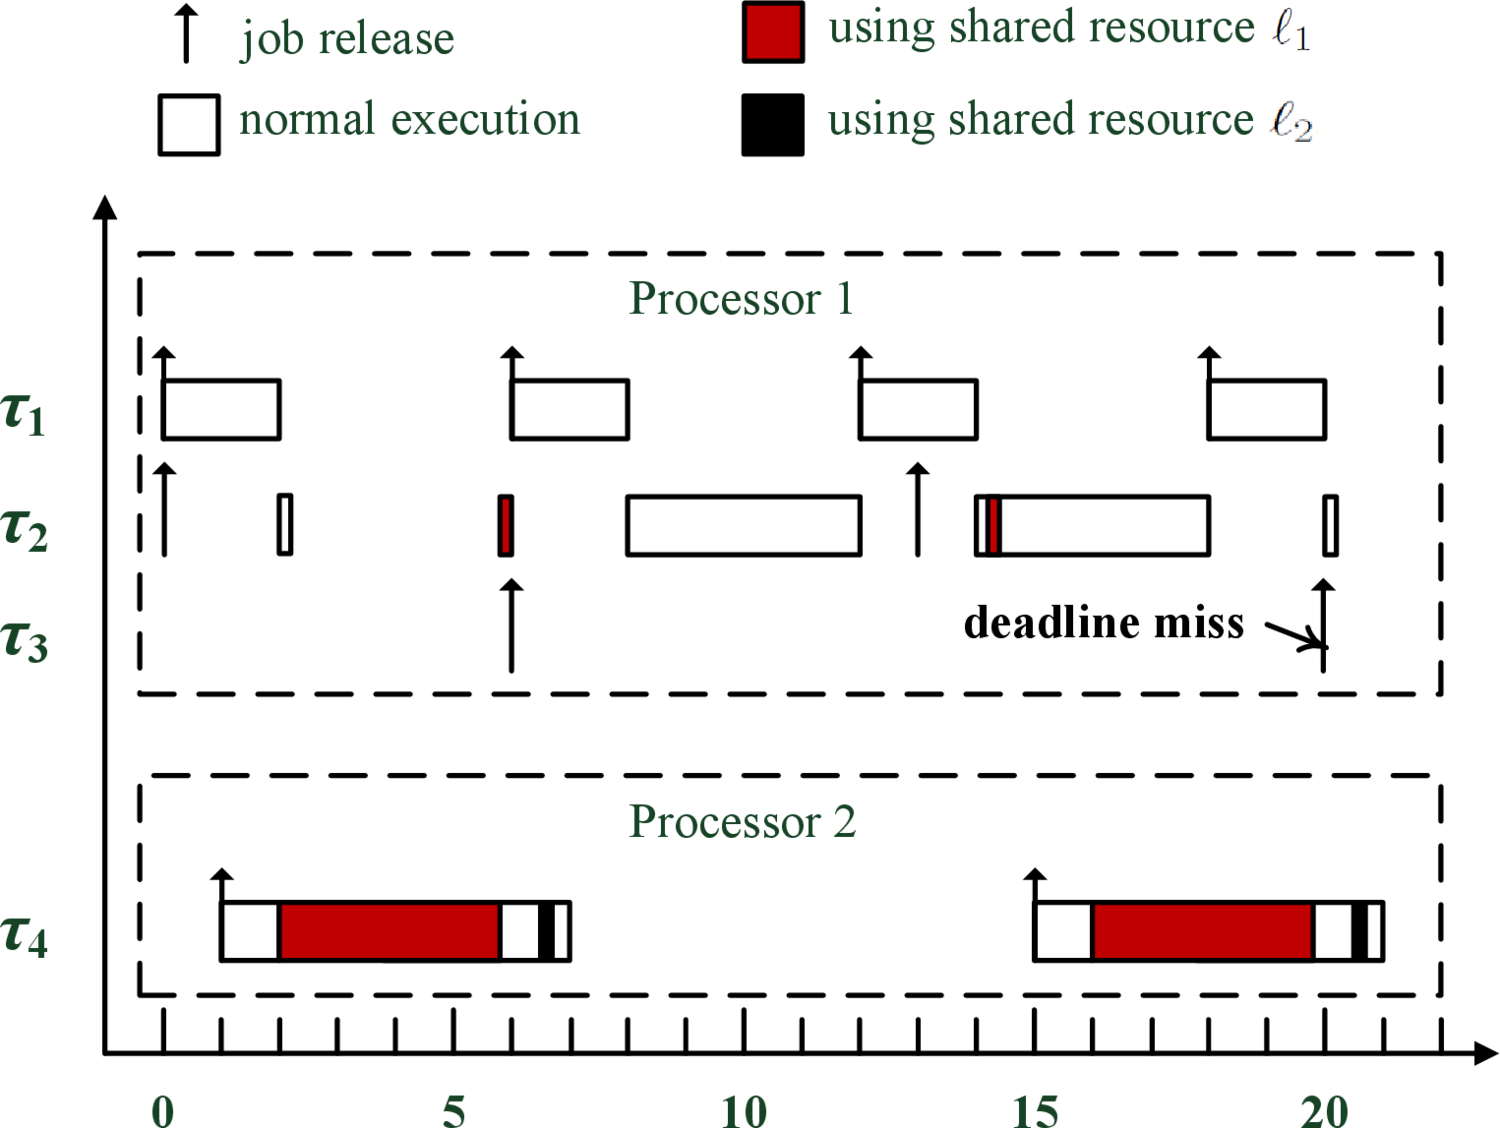
\includegraphics[width=12cm]{Counterexample}
\caption{An example schedule in which the first job of $\tau_3$ misses its deadline. 
}
\label{fig:counterexample}
\end{center}
\end{figure}

%\begin{figure}[!ht]
%\captionsetup{belowskip=-1pt}
%\begin{center}
%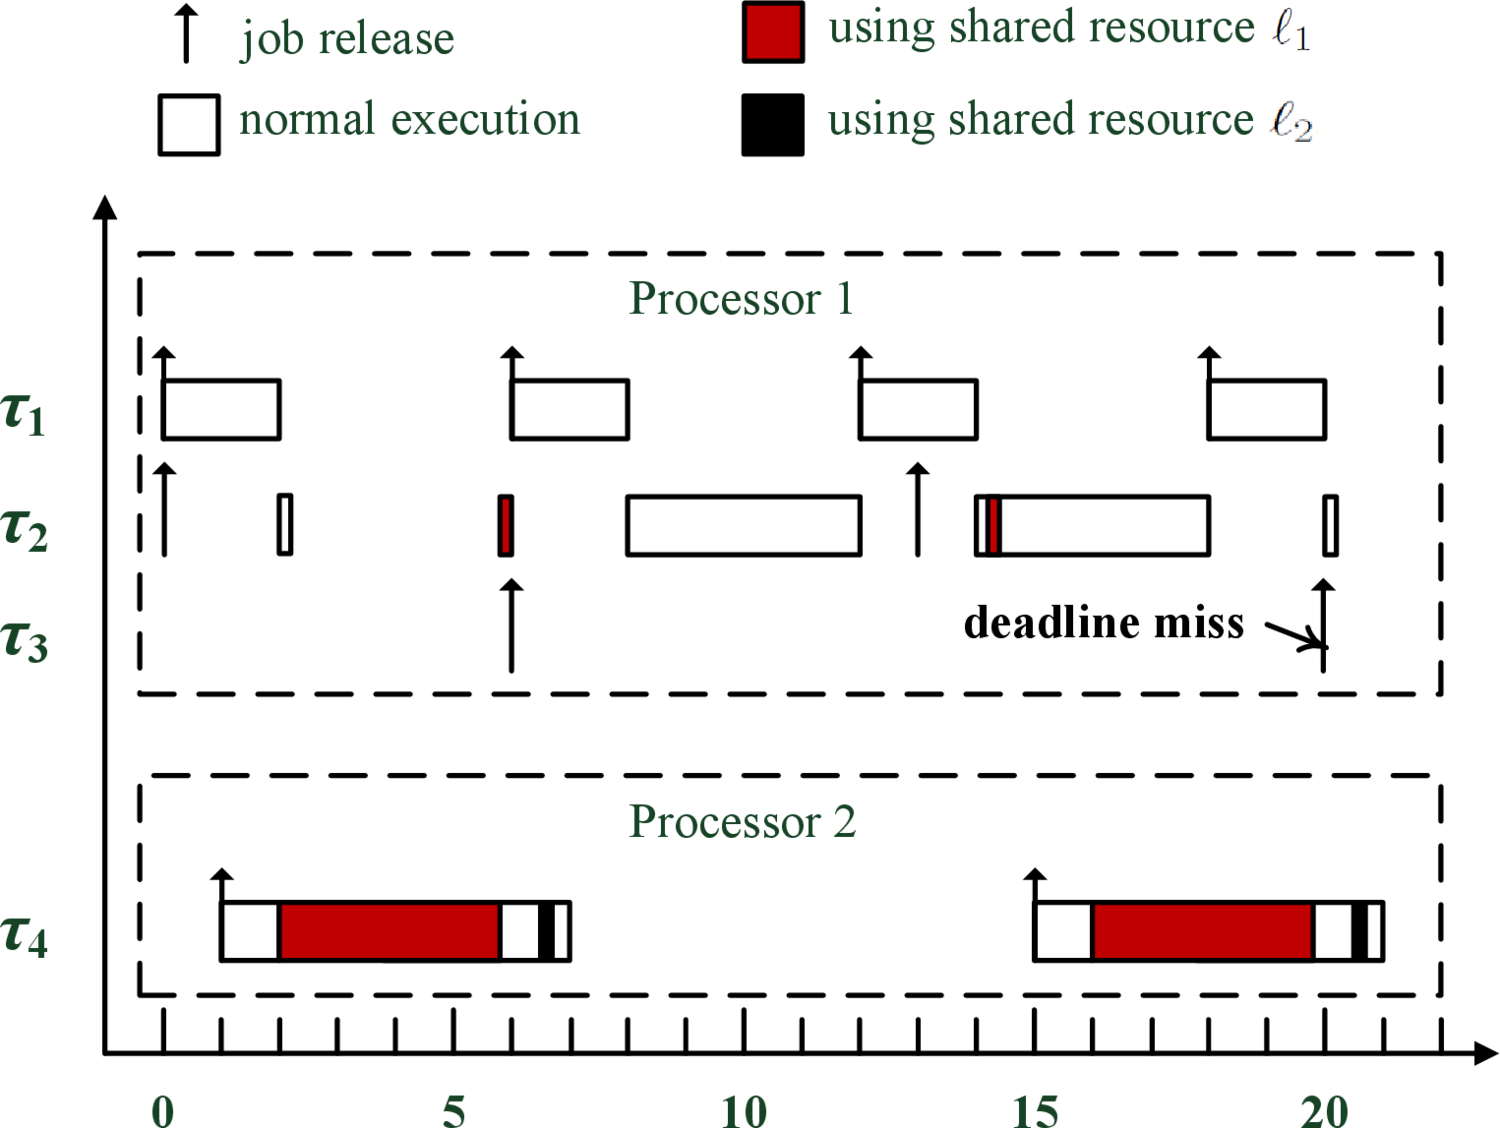
\includegraphics[width=12cm]{Counterexample}
%\caption{An example schedule in which $\tau_3$ misses a deadline. 
%}
%\label{fig:counterexample}
%\end{center}
%\end{figure}

\begin{table}
\centering
    \begin{tabular}{|c|c|c|c|c|c|c|} 
 \hline
        $\tau_k$ & $C_k$ & $T_k$ ($= D_k$) & $N_{k,1}$ & $L_{k,1}$ & $N_{k,2}$ & $L_{k,2}$\\
        \hline
        $\tau_1$ & 2             & 6  & 0 & 0 & 0 & 0\\ 
        $\tau_2$ & $4+2\epsilon$ & 13 & 1 & $\epsilon$ & 0 & 0\\
        $\tau_3$ & $\epsilon$    & 14 & 0 & 0 & 1 & $\epsilon$\\
        $\tau_4$ & 6             & 14 & 1 & $4-\epsilon$ & 1 & $\epsilon$ \\ 
        \hline
    \end{tabular}
    \caption{Task parameters}
    \label{table:parameters}
\end{table}

Consider four implicit deadline sporadic tasks ${\tau_1, \tau_2, \tau_3, \tau_4}$ (with parameters listed in Table \ref{table:parameters}, where $N_{k,1}$ ($N_{k,2}$) denotes the maximum number of requests that a job of $\tau_k$ can issue to resource $\res_1$ ($\res_2$), and $L_{k,1}$ ($L_{k,2}$) denotes the corresponding maximum critical section length), ordered by decreasing order of priority, that are scheduled on two processors using P-FP scheduling. $\tau_1$, $\tau_2$ and $\tau_3$ are assigned to processor 1, while $T_4$ is assigned to processor 2. Jobs of $\tau_2$ and $\tau_4$   each once access a shared resource $\res_1$  ($N_{2,1} = 1$ and $N_{4,1} = 1$). Jobs of $\tau_4$ each once access a shared resource $\res_2$ ($N_{4,2} = 1$). Each job of $\tau_2$ uses $\res_1$ for a duration of at most $L_{2,1} = \varepsilon < 1$ time units (an arbitrarily small quantity), and each job of $\tau_4$ uses $\res_1$ and $\res_2$ for at most $L_{4,1} = 4-\varepsilon$ and $L_{4,1} = \varepsilon$ time units respectively. 

Consider the response-time of $\tau_3$. Since $\tau_3$ is the lowest-priority task on its processor, it does not incur any local blocking (\ie,$s_3 \sum_{\tau_l \in \fun{lp}(3) \cap P(\tau_3)} \max_{1 \leq j < s_l} C_{l,j}^{\prime} = 0$). While each time $\tau_3$ requests $\res_2$, it may be delayed by $\tau_4$ for at most $\epsilon$. Thus, the maximum remote blocking of $\tau_3$ is bounded by $B_3^r = \epsilon$ \footnote{In general, the upper bound on blocking of course depends on the specific locking protocol in use, but in this example, by construction, the stated bound holds under any reasonable locking protocol. Recent surveys of multiprocessor semaphore protocols may be found in \cite{bbb-2013,yang-2015}.}. With regard to the remote blocking incurred by each higher-priority task, we have $B_1^r = 0$ because $\tau_1$ does not request any global resource. Further, each time when a job of $T_2$ requests $\res_1$, it may be delayed for a duration of at most $4-\varepsilon$, thus $B_2^r = 4-\varepsilon$. Therefore, according to Eq. \ref{eqn:wcrt}, we have
\begin{align*}
& R_3^0 = \varepsilon + \varepsilon = 2\varepsilon, \\
& R_3^1 = 2\varepsilon + 0 + \left \lceil \frac{2\varepsilon + 0}{6} \right \rceil \cdot 2 + \left \lceil \frac{2\varepsilon + 4 - \varepsilon}{13} \right \rceil \cdot (4+2\varepsilon) =  6+4\varepsilon, \\
& R_3^2 = 2\varepsilon + 0 + \left \lceil \frac{6+4\varepsilon + 0}{6} \right \rceil \cdot 2 + \left \lceil \frac{6+4\varepsilon + 4-\varepsilon}{13} \right \rceil \cdot (4+2\varepsilon) = 8+4\varepsilon, \\
& R_3^3 = 2\varepsilon + 0 + \left \lceil \frac{8+4\varepsilon + 0}{6} \right \rceil \cdot 2 + \left \lceil \frac{8+4\varepsilon + 4-\varepsilon}{13} \right \rceil \cdot (4+2\varepsilon) = 8+4\varepsilon.
\end{align*}
 
As a result, $R_3 = 8+4\varepsilon < 14 = D_3$, and $\tau_3$ is considered to be schedulable according to the analysis in \cite{lakshmanan-2009}. However, there exists a schedule, shown in Fig. \ref{fig:counterexample}, where $\tau_3$  actually misses a deadline at time~20, which implies that the analysis framework in \cite{lakshmanan-2009} is too optimistic (in certain cases). 

\subsection{Incorrect Time Request Analysis With Global Resource Sharing}

Besides the over-optimistic problem found in \cite{lakshmanan-2009}, a straightforward adoption of the traditional time request analysis with global resource sharing is also not safe, as we show next.

 In \cite{NBN:11}, an \emph{interface-based analysis} based on the time request analysis was derived for real-time open systems, where each processor contains a task set and the tasks on different processors may share global resources. Intuitively, the interface abstracts the requirements of global resource sharing on each processor that should be satisfied to guarantee the schedulability of the system in the processor. In particular, the maximum blocking time that a task $\tau_k$ can tolerate without missing its deadline, denoted by $\fun{mtbt}_k$, is evaluated as following. 

Starting from the schedulability condition, $\tau_k$ is considered schedulable in a single processor if

\begin{equation}
\label{eqn:rbf-1}
\exists t \in (0,D_k]: \fun{rbf_{FP}}(k,t) \leq t, 
\end{equation}
where $\fun{rbf_{FP}}(k,t)$ is the \emph{request bound function} of $\tau_k$, which is computed by

\begin{equation}
\label{eqn:rbf-2}
\fun{rbf_{FP}} = C_k + B_k + \sum_{\tau_i \in \fun{hp}(k)} \left \lceil \frac{t}{T_i} \right \rceil \cdot C_i.
\end{equation}

In Eq. \ref{eqn:rbf-2}, $B_k$ denotes the total blocking time of $\tau_k$. By substituting $B_k$ and $\fun{mtbt}_k$, $\fun{mtbt}_k$ is then computed by

\begin{equation}
\label{eqn:bloc-tolerate}
\fun{mtbt}_k = \max_{0<t \leq D_k} \left( t - ( C_k + \sum_{\tau_i \in \fun{hp}(k)} \left \lceil \frac{t}{T_i} \right \rceil \cdot C_i ) \right).
\end{equation}

However, from the discussion in section \ref{sec:counterexample} we can already infer that the analysis used in Eq. \ref{eqn:rbf-1} and Eq. \ref{eqn:rbf-2}, which ignores the effects of remote blocking on interference and quantifies the total interference from a task $\tau_i$ on $\tau_k$ over a duration of length $t$ as $\left \lceil \frac{t}{T_i} \right \rceil \cdot C_i$, is over optimistic. 

Consider $\tau_3$ in the previous example (with parameters listed in Table \ref{table:parameters}). According to Eq. \ref{eqn:bloc-tolerate}, $\fun{mtbt}_3$ is $12 - (\epsilon + \lceil 12 / 6 \rceil \cdot 2 + \lceil 12 / 13 \rceil \cdot (4+2\epsilon)) = 4-3\epsilon$ (when $t=12$), which implies that $\tau_3$ can tolerate a maximum blocking time of at least $4-3\epsilon$ without missing its deadline. However, this is not true since $\tau_3$ is unschedulable even without incurring any blocking, as shown in Fig. \ref{fig:counterexample}.

\subsection{A Safe Response Time Bound}
\label{sec:safe_bound}

In Eq. \ref{eqn:wcrt}, the remote blocking of each higher-priority task (\ie, $B_i^r$) is counted in a similar way as release jitter. However, it is not sufficient to count the duration of remote blocking as release jitter, as already explained in section XXX. A straightforward fix is thus to replace $B_i^r$, in the ceiling function (\ie, the second term in Eq. \ref{eqn:wcrt}), with a larger value such as $D_i$ (as proved/discussed in section XXX) or $R_i - C_i$ (as proved / discussed in section XXX). Similarly, replacing $\sum_{\tau_i \in \fun{hp}(k)} \lceil t / T_i \rceil \cdot C_i$ in Eq. \ref{eqn:rbf-2} and Eq. \ref{eqn:bloc-tolerate} with $\sum_{\tau_i \in \fun{hp}(k)} \lceil (t+D_i) / T_i \rceil \cdot C_i$ or $\sum_{\tau_i \in \fun{hp}(k)} \lceil (t+R_i-C_i) / T_i \rceil \cdot C_i$ may fix the over-optimistic problem in \cite{NBN:11}.

Further, since most papers reviewed in section \ref{sec:papers} merely reused the over-optimistic analysis approach introduced in \cite{lakshmanan-2009}, the stated fix may be used to correct the response-time tests in these papers.
\section{Soft Real-Time Self-Suspending Task Systems}
\label{sec:soft-realtime}

The goal of real-time scheduling is to guarantee timing predictability; in other words, every task is schedulable if it meets the predefined timing constraints at design time. Being ``schedulable'' depends on whether task deadlines are hard or soft. 
For a hard real-time (HRT) task, its deadline must be met; while for a soft real-time (SRT) task, missing some deadlines can be tolerated. We assume a well-studied SRT notion that a SRT task is schedulable if its tardiness can be provably bounded. (Such bounds would be expected to be reasonably small.) A task's tardiness is defined to be its maximum job tardiness, which is calculated by a job's completion time minus the job's absolute deadline.

The schedulability analysis techniques on soft real-time self-suspending task systems can be categorized into two categories: suspension-oblivious analysis v.s. suspension-aware analysis.

\subsection{Suspension-oblivious analysis}
\label{sec:sus-oblivious-soft}

 The suspension-oblivious analysis simply treat all suspension as computation. From \cite{Devi2005,Leontyev072}, tardiness is bounded under a pure computational task system (no suspensions) provided $U_{sum} \leq m$ where $U_{sum}$ is the total utilization. A downside of treating all suspensions as computation is that this causes utilizations to be higher, which in many cases may cause total utilization to exceed $m$, where $m$ is the number of processors in the system.  This suspension-oblivious approach causes an $O(n)$ utilization loss, where $n$ denotes the number of self-suspending tasks in the system. 
 Due to the $O(n)$ utilization loss, the suspension-oblivious analysis is pessimistic. 

\subsection{Suspension-aware analysis}
\label{sec:sus-aware-soft}

Several recent works have been conducted to reduce this utilization loss by focusing on deriving suspension-aware analysis. The main difference between the suspension-aware and the suspension-oblivious analysis is that, under the suspension-aware analysis, suspensions are specifically considered in the task model as well as in the schedulability analysis. These works on conducting suspension-aware analysis techniques for soft real-time suspending task systems on multiprocessors are mainly done by Liu and Anderson~\cite{Liu3,Liu4,Liu5,Liu9,Liu11}. The main idea behind these techniques is that treating all suspensions as computation is pessimistic, instead, smartly treating a selective minimum set of suspensions as computation can significantly reduce the pessimism in the schedulability analysis. This is also the main reason why these techniques significantly improve upon the suspension-oblivious approach in most cases, and some of these techniques analytically dominate the suspension-oblivious approach, as to be briefly reviewed next.

In 2009, Liu and Anderson derived the first such schedulability test~\cite{Liu3}, where they showed that in fully-preemptive sporadic systems, bounded tardiness can be ensured by developing suspension-aware analysis under GEDF and GFIFO. Specifically it is shown in \cite{Liu3} that tardiness in such a system is bounded provided 
\begin{equation}\label{eq:constraint} U_{sum}^s + U_L^c < (1-\xi_{max}) \cdot m , \end{equation}
where $U_{sum}^s$ is the total utilization of all self-suspending tasks, $c$ is the number of computational tasks (which do not self-suspend), $m$ is the number of processors, $U_L^c$ is the sum of the $\min(m-1,c)$ largest computational task utilizations, and $\xi_{max}$ is a parameter ranging over $[0,1]$ called the \textit{maximum suspension ratio}, which is defined to be the maximum value among all tasks' suspension ratios. For any task $T_i$, its suspension ratio, denoted $\xi_i$, is defined to be $\xi_i = \dfrac{s_i}{s_i+e_i}$, where $s_i$ is $T_i$'s suspension length and $e_i$ is its execution cost.  Significant utilization loss may occur when using (\ref{eq:constraint}) if $\xi_{max}$ is large. Unfortunately, it is unavoidable that many self-suspending task systems will have large $\xi_{max}$ values. For example, consider a task system with three tasks scheduled on two processors: $T_1$ has an execution cost of 5, a suspension length of 5, and a period of 10, $T_2$ has an execution cost of 2, a suspension length of 0, and a period of 8, and $T_3$ has an execution cost of 2, a suspension length of 2, and a period of 8. For this system, $U_{sum}^s = u_1+u_3= \dfrac{5}{10} + \dfrac{2}{8} = 0.75$, $U_L^c = u_2 = \dfrac{2}{8} = 0.25$, $\xi_{max} = \xi_1 = \dfrac{5}{5+5} = 0.5$. Although the total utilization of this task system is only half of the overall processor capacity, it is not schedulable using the prior analysis since it violates the utilization constraint in (\ref{eq:constraint}) (since $U_{sum}^s+U_L^c =1=(1-\xi_{max}) \cdot m$).

In a follow-up work \cite{Liu5}, by observing that the utilization loss seen in (\ref{eq:constraint}) is mainly caused by a large value of $\xi_{max}$, Liu and Anderson present a technique that can effectively decrease the value of this parameter, thus increasing schedulability. They show that this can be done by treating \textit{partial} suspensions as computation. That is, they consider intermediate choices between the two currently-available extremes of treating \textit{all} (as is commonly done) or \textit{no} (using the analysis in ???Liu093) suspensions as computation. This approach is often able to decrease $\xi_{max}$ at the cost of at most a slight increase in the left side of (\ref{eq:constraint}). The authors present both a linear programming solution for determining how much suspension time to be treated as computation as well as an optimal algorithm that runs in $O((N^s)^2)$ time, where $N^s$ is the number of self-suspending tasks. The authors analyze the schedulability improvement brought by the proposed approach via an experimental study involving randomly-generated task systems. In all scenarios considered in this study, this approach was able to improve schedulability, and in most scenarios, by a substantial margin. 

In \cite{Liu4}, Liu and Anderson  show that any task system with self-suspensions, pipelines, and
non-preemptive sections can be transformed for analysis purposes into a system with only self-suspensions \cite{Liu4}. The transformation process treats delays caused by pipeline-based precedence constraints and non-preemptivity as self-suspension delays.
In \cite{Liu9,Liu11}, Liu and Anderson derive the first soft real-time schedulability test for suspending task systems that analytically dominates the suspension-oblivious approach. Specifically, they show that an $O(M)$ utilization loss (where $M$ is the number of processors) can be achieved under a new suspension-aware analysis technique. 



%%% Local Variables:
%%% mode: latex
%%% TeX-master: "JRTS/JRTS.tex"
%%% End:


  
\section{Hardness Review of Self-Suspending Task Models}
\label{sec:hardness}
This section reviews the hardness for designing scheduling algorithms and schedulability analysis of self-suspending task systems. Table \ref{table:complexity} summarizes the complexity classes of the corresponding problems, in which the complexity problems are reviewed according to the considered task models (\ie, segmented or dynamic self-suspending models) and the scheduling strategies (\ie, fixed- or dynamic-priority scheduling). Notably, for self-suspending task systems, only the complexity class for verifying the existence of a feasible schedule for segmented tasks is proved in the literature~\cite{Ric03,Ridouard_2004}, most corresponding problems are still open.

\begin{table}
\centering
    \begin{tabular}{|c|c|c|c|c|}
 \hline
        Task Model & Feasability & \multicolumn{3}{c|}{Schedulability} \\
        \hline
        &  & Fixed-Priority & \multicolumn{2}{c|}{Dynamic-Priority}\\
        &  & Scheduling     & \multicolumn{2}{c|}{Scheduling}\\
        \cline{3-5}    
        Segmented Self- & ${\cal NP}$-hard in &  & Constrained & Implicit\\
        Suspension  & the strong &   & Deadlines   & Deadlines \\
        \cline{4-5}
        Models & sense \cite{Ridouard_2004} & unknown & at least co${\cal NP}$- & co${\cal NP}$-hard \\
        &  & & hard in the & in the strong\\
        & & & strong sense & sense\\
        \hline
        Dynamic Self- & \multirow{3}{*}{unknown} & & at least co${\cal NP}$- & \multirow{3}{*}{unknown}\\
        Suspension & & unknown &hard in the & \\
        Models & & & strong sense & \\
        \hline
    \end{tabular}
    \caption{The complexity classes of scheduling and schedulability analysis for self-suspending tasks}
    \label{table:complexity}
\end{table}

\subsection{Hardness for Scheduling Segmented Self-Suspending Tasks}
Verifying the existence of a feasible schedule for segmented self-suspending task systems is proved to be ${\cal NP}$-hard in the strong sense in \cite{Ridouard_2004} for implicit-deadline tasks with at most one self-suspension per task. For this model, it is also shown that EDF and RM do not have any speedup factor bound in in \cite{Ridouard_2004} and \cite{RTSS-ChenL14}, respectively. The generalization of the segmented self-suspension model to multi-threaded tasks (i.e., every task is defined by a Directed Acyclic Graph with edges labelled by suspension delays), the feasibility problem is also known to be  ${\cal NP}$-hard in the strong sense  \cite{Ric03} even if all subjobs have unit execution times. 

The only results with speedup factor analysis for fixed-priority scheduling and dynamic priority scheduling can be found in \cite{RTSS-ChenL14} and \cite{WC16-suspend-DATE}. The analysis with speedup factor $3$ in \cite{RTSS-ChenL14} can be used for systems with at most one self-suspension interval per task in dynamic priority scheduling. The analysis with a bounded speedup factor in \cite{WC16-suspend-DATE} can be used for fixed-priority and dynamic-priority systems with any number of self-suspension intervals per task. However, the speedup factor in \cite{WC16-suspend-DATE} depends on, and grows quadratically with respect to the number of self-suspension intervals. Therefore, it can only be \emph{practically} used when there are only a few number of suspension intervals per task. The scheduling policy used in \cite{WC16-suspend-DATE} is \emph{laxity-monotonic} (LM) scheduling, which assigns the highest priority to the task with the least laxity, that is, $D_i-S_i$.

With respect to this scheduling problem, there was no theoretical lower bound (with respect to the speedup factors) of this scheduling problem. 


The above analysis also implies that the priority assignment in fixed-priority scheduling should be carefully designed. Traditional approaches like RM or EDF do not work very well. LM may work for a few self-suspending intervals, but how to perform the optimal priority assignment is an open problem. Such a difficulty comes from scheduling anomalies that may occur at run-time. In \cite{Ridouard_2004} is shown using a simple counter example that reducing execution times or self-suspension delays can lead some task to miss deadlines under EDF (i.e., EDF is no longer sustainable). This latter result can be easily extended to static schdeling policies (i.e., RM and DM). Lastly, in \cite{RidouardR06}, it is proved that no deterministic online scheduler can be optimal if the real-time tasks are allowed to suspend themselves.


\subsection{Hardness for Scheduling Dynamic Self-Suspending Tasks}
The complexity class for verifying the existence of a feasible schedule for dynamic self-suspending task systems is unknown in the literature. The proof in \cite{Ridouard_2004} cannot be applied to this case. 
It is proved in \cite{huangpass:dac2015} that the speed-up factor for RM, DM, and LM scheduling is $\infty$. Here, we repeat the example in \cite{huangpass:dac2015}. Consider the following implicit-deadline task set with one self-suspending task and one sporadic task:
\begin{itemize}
 \setlength\itemsep{0em}
\item $C_1=1-2\epsilon$, $S_1=0$, $T_1=1$
\item  $C_2=\epsilon$, $S_2=T-1-\epsilon$, $T_2=T$
\end{itemize}
where $T$ is any natural number larger than $1$ and $\epsilon$ can be arbitrary small.

It is clear that this task set is schedulable if we assign higher priority to
task $\tau_2$.
Under either RM, DM, and LM scheduling, task $\tau_1$ has higher priority than task $\tau_2$. It was proved in \cite{huangpass:dac2015} that this example has a speed-up factor $\infty$ when $\epsilon$ is close to $0$.

There is no upper bound of this problem in the most general case. The analysis in \cite{huangpass:dac2015} for a speedup factor $2$ uses a trick to compare the speedup factor with respect to the \emph{optimal fixed-priority schedule} instead of the \emph{optimal schedule}. There is no proof or evident to show that this factor $2$ is also the factor when the reference is the \emph{optimal schedule}.

With respect to this problem, there was no theoretical lower bound (with respect to the speedup factors) of this scheduling problem. 


The above analysis also implies that the priority assignment in fixed-priority scheduling should be carefully designed. Traditional approaches like RM or EDF do not work very well. LM also does not work well. The priority assignment used in \cite{huangpass:dac2015} is based on the optimal-priority algorithm (OPA) from Audsley \cite{audsley-1993} with an OPA-compatible schedulability analysis. However, since the schedulability test used in \cite{huangpass:dac2015}  is not exact, the priority assignment is also not the optimal solution.
Finding the optimal priority assignment here is also an open problem.


\subsection{Hardness for Schedulability Tests for Segmented Self-Suspension}
\paragraph{Preemptive Fixed-Priority Scheduling:}   
For this case, the complexity class of verifying whether the worst-case response time is no more than the relative deadline is \emph{unknown} up to now. The evidence provided in \cite{ecrts15nelissen} also suggests that this problem may be very difficult even for a task system with \emph{only one self-suspending task}. The solution in \cite{ecrts15nelissen}  requires exponential time complexity for $n-1$ sporadic tasks and 1 self-suspending task. The other solutions \cite{Huang:multiseg}\cite{PH:rtss98} require pseudo-polynomial time complexity but are only sufficient schedulability tests.

The lack of something like the critical instant theorem in the ordinary sporadic task systems to reduce the search space of the worst-case behaviour has led to the complexity explosion to test exponential combinations of release patterns. The complexity class is at least as hard as the ordinary sporadic task systems under fixed-priority scheduling. It is shown in \cite{EisenbrandR08} that the response time analysis is at least weakly NP-hard and the complexity class of the schedulability test is unknown.
Whether the problem (with segmented self-suspension) is ${\cal NP}$-hard in the strong or weak sense is an open problem.

\paragraph{Preemptive Dynamic-Priority Scheduling:} 
For this case, if the task systems are with constrained deadlines, i.e., $D_i \leq T_i$, the complexity class of this problem is at least co${\cal NP}$-hard in the strong sense, since a special case of this problem is co${\cal NP}$-complete in the strong sense \cite{DBLP:conf/ecrts/Ekberg015}. It has been proved in \cite{DBLP:conf/ecrts/Ekberg015} that verifying uniprocessor feasibility of sporadic tasks with constrained deadlines is strongly co${\cal NP}$-complete.  Therefore, when we consider constrained-deadline self-suspending task systems, the complexity class is at least co${\cal NP}$-hard in the strong sense.

It is also not difficult to see that the implicit-deadline case is also at least co${\cal NP}$-hard.  A special case of segmented self-suspending task system is to allow a task $\tau_i$ having exactly one self-suspension interval with a \emph{fixed} length $S_i$ and one computation segment with WCET $C_i$. Therefore, the relative deadline of the computation segment of task $\tau_i$ (after it is released to be scheduled) is $D_i = T_i-S_i$. Therefore, the implicit-deadline segmented self-suspending task system is equivalent to a constrained-deadline task system, which is co${\cal NP}$-complete in the strong sense. Since a special case of the problem is co${\cal NP}$-complete in the strong sense, the problem is co${\cal NP}$-hard in the strong sense.


\subsection{Hardness for Schedulability Tests for Dynamic Self-Suspension}
\paragraph{Preemptive Fixed-Priority Scheduling:}   

Similarly, for this case, with dynamic self-suspension, the complexity class of verifying whether the worst-case response time is no more than the relative deadline is \emph{unknown} up to now. There is \emph{no exact} schedulability analysis for this problem up to now. The solutions in \cite{Liu:2000:RS:518501}\cite{LiuChen:rtss2014}\cite{huangpass:dac2015} are only sufficient schedulability tests. 

The lack of something like the critical instant theorem and the dynamics of the dynamic self-suspending behaviour have constrained the current researches to provide exact schedulability tests. The complexity class is at least as hard as the ordinary sporadic task systems under fixed-priority scheduling. It is shown in \cite{EisenbrandR08} that the response time analysis is at least weakly NP-hard and the complexity class of the schedulability test is unknown. Whether the problem (with dynamic self-suspension) is ${\cal NP}$-hard in the weak or strong sense is an open problem.

\paragraph{Preemptive Dynamic-Priority Scheduling:} 
For this case, if the task systems are with constrained deadlines, i.e., $D_i \leq T_i$, similarly, the complexity class of this problem is at least co${\cal NP}$-hard in the strong sense, since a special case of this problem is co${\cal NP}$-complete in the strong sense \cite{DBLP:conf/ecrts/Ekberg015}. For implicit-deadline self-suspending task systems, the schedulability test problem is not well-defined, since there is no clear scheduling policy that can be applied and tested. Therefore, we would conclude this as an open problem.

\section{Other Remarks}

\subsection{Some Inherited Errors}





\subsection{Rule of Thumb to Handle Self-Suspending Task Systems}



%%% Local Variables:
%%% mode: latex
%%% TeX-master: "JRTS/JRTS.tex"
%%% End:


  
\mychapter{Final Discussion}
%\subsection{Summary}  
 Self-suspending behavior is becoming an increasingly prominent
characteristic in real-time systems, for example: (i) I/O-intensive systems
(ii) multi-processor synchronization and scheduling, and (iii)
computation offloading with coprocessors, like graphics processing
units (GPUs).  This paper has reviewed the literature in the light of
recent developments in the analysis of self-suspending tasks,
explained the general methodologies, summarized the computational complexity classes, 
and detailed a number of 
misconceptions in the literature concerning this topic. We
have given concrete examples to demonstrate the effect of these
misconceptions, listed some flawed statements in the literature, and
presented potential solutions. These misconceptions include:
\begin{itemize}
\item Incorrect quantification of jitter for dynamic self-suspending
  task systems, which was used in
  \cite{ECRTS-AudsleyB04,RTAS-AudsleyB04,RTCSA-KimCPKH95,MingLiRTCSA1994}.  This
  misconception was unfortunately adopted in
  \cite{zeng-2011,bbb-2013,yang-2013,kim-2014,han-2014,carminati-2014,yang-2014,lakshmanan-2009} to analyze the worst-case response time for
  partitioned multiprocessor real-time locking protocols.
\item Incorrect quantification of jitter for segmented self-suspending
  task systems, which was used in  \cite{RTCSA-BletsasA05}.
\item Incorrect assumptions for a critical instant with
  synchronous releases, which was used in \cite{LR:rtas10}.
\item Incorrectly counting highest-priority self-suspending time to reduce the
  interference on the lower-priority tasks, which was used in  \cite{RTSS-KimANR13}. 
\item Incorrect segmented fixed-priority scheduling with period
  enforcement, which was used in
  \cite{RTSS-KimANR13,DBLP:journals/ieicet/DingTT09}.
\item Incorrect conversion of higher-priority self-suspending tasks into sporadic tasks with release jitter, which was used in \cite{ecrts15nelissen}.
\end{itemize}
For completeness, all the misconceptions, open issues, closed issues,
and inherited flaws discussed in this paper are listed in Table~\ref{tab:summary}.

This review extensively references errata and reports as follows:
the proof \cite{ChenHuangNelissen} of the correctness of the
analysis by Jane W.S. Liu in her book \cite[Page
164-165]{Liu:2000:RS:518501}; the re-examination and the limitations
\cite{ChenBrandenburg} of the period enforcer algorithm proposed in
\cite{Raj:suspension1991}; the erratum report \cite{BletsasReport2015}
of the misconceptions in
\cite{ECRTS-AudsleyB04,RTAS-AudsleyB04,RTCSA-BletsasA05}; and the erratum \cite{Kim2016} of the
misconceptions in \cite{RTSS-KimANR13}. 
For brevity, these errata and reports are only summarized in
this review. We encourage the readers to refer to these reports and
errata for more detailed explanations.



\begin{table}[t]
  \centering
\scalebox{0.8}{
\begin{tabular}{||C{3cm}|L{7cm}||C{3cm}|C{2cm}|}  
  \hline
  \hline
  Type of Arguments& Affected papers and statements &
  Potential Solutions & (flaw/issue) status\\
  \hline
  \multirow{6}{*}{Conceptual Flaws} & \cite{ECRTS-AudsleyB04,RTAS-AudsleyB04}: Wrong
  quantification of jitter& See Section~\ref{sec:wrong-jitter-dynamic} or the
  erratum filed by the authors \cite{BletsasReport2015}& solved\\
  \cline{2-4}
  & \cite{MingLiRTCSA1994}:   Wrong quantification of jitter & See Section
  \ref{sec:wrong-jitter-dynamic} & solved\\
  \cline{2-4}
  & \cite{RTCSA-BletsasA05}:   Wrong quantification of jitter & See Section
  \ref{sec:wrong-jitter-segmented} or \cite{BletsasReport2015}& solved\\
  \cline{2-4}
  & \cite{LR:rtas10}:  Critical instant theorem in Section III and the
  response time analysis are incorrect & See Section
  \ref{sec:wrong-critical} or \cite{ecrts15nelissen} & solved\\
  \cline{2-4}
  & \cite{RTSS-KimANR13}: Incorrect accounting for the highest-priority
  interference in Theorems 2 and 3 & See
  Section~\ref{sec:wrong-highest-priority} & solved\\
  \cline{2-4}
  & \cite{RTSS-KimANR13,DBLP:journals/ieicet/DingTT09}: Wrong schedulability test for segmented
  fixed-priority scheduling with periodic enforcement (Section IV
  in \cite{RTSS-KimANR13}, Section 3 in \cite{DBLP:journals/ieicet/DingTT09})& See Section~\ref{sec:wrong-periodic} &
  not solved\\
  \cline{2-4}
  & \cite{ecrts15nelissen}: Incorrect combination of techniques in Section VI by using release
  jitter without converting suspension into 
  computation & See Section~\ref{sec:wrong-jitter-convert-sporadic}&
  solved\\
  \cline{2-4}
  \hline
  \multirow{2}{*}{Inherited Flaws} &
  \cite{RTCSA-KimCPKH95,zeng-2011,bbb-2013,yang-2013,kim-2014,han-2014,carminati-2014,yang-2014,lakshmanan-2009}:
  Adopting wrong quantifications of jitters (refer to
  Section~\ref{sec:syn} in this paper)& See
  Section~\ref{sec:safe_bound} & solved\\
  \cline{2-4}
  & \cite{DBLP:conf/ecrts/LiuA13}: Inherited flaw from
  \cite{DBLP:conf/rtss/GuanSYY09} and unsafe Lemma 1 to quantify the workload& See the erratum
  \cite{erratu-cong-anderson} filed by the authors & solved\\
  \hline
  \multirow{2}{*}{Closed Issues} & \cite[Page
  164-165]{Liu:2000:RS:518501}: schedulability test without any proof & See
  \cite{ChenHuangNelissen} for a proof& solved\\
  \cline{2-4}
  &\cite{Raj:suspension1991}: period enforcer can be used for
  deferrable task systems. It may result in deadline
  misses for self-suspending tasks and is not compatible with multiprocessor synchronization & See
  \cite{ChenBrandenburg} for the explanations.& solved\\
  \hline
  \multirow{2}{*}{Open Issues} &  \cite{DBLP:conf/ecrts/Devi03}: Proof
  of Theorem
  8  for considering suspension as blocking in EDF is incomplete& ?& ?\\
  \cline{2-4}
  & \cite{LR:rtas10}: Proofs for slack enforcement in Sections IV and V
  are incomplete & ?& ?\\
  \hline
  \hline
\end{tabular}}
\vspace{0.1in}
  \caption{List of flaws/incompleteness and their solutions in the
    literature. All the references to Section X in the column
    ``Potential Solutions'' are listed for this paper.}
  \label{tab:summary}
\end{table}


\mysection{Open Issues in the Existing Results}
\label{sec:open-issues-existing}  
We have carefully re-examined the results related to self-suspending
real-time tasks in the literature in the past 25 years. However, there
are also some results in the literature that may require further
elaborations. These include the following results in the literature:
\begin{itemize}
\item Devi (in Theorem 8 in \cite[Section
  4.5]{DBLP:conf/ecrts/Devi03}) extended the analysis proposed by Jane
  W.S. Liu in her book \cite[Page 164-165]{Liu:2000:RS:518501} to
  EDF scheduling. This method quantifies the additional interference
  due to self-suspensions from the higher-priority jobs by setting up
  the \emph{blocking time} induced by self-suspensions. However, there
  is no formal proof in \cite{DBLP:conf/ecrts/Devi03}. The proof made
  by Chen et al. in \cite{ChenHuangNelissen,ChenECRTS2016-suspension} for fixed-priority
  scheduling cannot be directly extended to EDF scheduling. The
  correctness of Theorem 8 in \cite[Section
  4.5]{DBLP:conf/ecrts/Devi03} should be supported with a rigorous
  proof, since self-suspension behavior has induced several
  non-trivial phenomena.

\item For segmented self-suspending task systems with at most one
  self-suspending interval, Lakshmanan and Rajkumar proposed two slack
  enforcement mechanisms in \cite{LR:rtas10} to shape the demand of a
  self-suspending task so that the task behaves like an ideal ordinary
  periodic
  task.  From the scheduling point of view, this means that there is
  no \emph{potential} scheduling penalty when analyzing the interferences of the
  higher-priority tasks. However, the suspension time of the task under
  analysis has to be converted into computation. The correctness of the dynamic slack
  enforcement in \cite{LR:rtas10} is heavily based on the statement of Lemma
  4 in \cite{LR:rtas10}. However, the proof is not rigorous for the
  following reasons:
  \begin{itemize}
  \item Firstly, the proof argues: ``\emph{Let the duration $R$ under
    consideration start from time $s$ and finish at time $s +
    R$. Observe that if $s$ does not coincide with the start of the
    Level-$i$ busy period at $s$, then $s$ can be shifted to the left
    to coincide with the start of the Level-$i$ busy period. Doing so
    will not decrease the Level-$i$ interference over $R$.}'' This
    argument has to be proved by also handling cases in which a task
    may suspend before the $Level-i$ busy period. This results in the
    possibility that a higher-priority task $\tau_j$ starts with the
    second computation segment in the Level-$i$ busy
    period. Therefore, the first and the third paragraphs in the proof
    of Lemma 4 \cite{LR:rtas10} require more rigorous reasoning.

  \item Secondly, the proof argues: ``\emph{The only property
      introduced by dynamic slack enforcement is that under worst-case
      interference from higher-priority tasks there is no slack
      available to $J_j^p$ between $f_j^p$ and $\rho_j^p + R_j$.
      $\ldots$ The second segment of $\tau_j$ is never delayed under
      this transformation, and is released sporadically.} '' In fact,
    the slack enforcement may make the second computation segment
    arrive earlier than its worst-case. For example, we can greedily
    start with the worst-case interference of task $\tau_j$ in the
    first iteration, and do not release the higher-priority tasks
    (higher than $\tau_j$) after the arrival of the second job of task
    $\tau_j$. This can immediately create some release jitter of the
    second computation segment $C_j^2$.
  \end{itemize}
  With the same reasons, the static slack enforcement algorithm in
  \cite{LR:rtas10} also requires a more rigorous proof.
\end{itemize}

\mysection{Potentially Correct Approaches}
\label{sec:correct-solutions} 

We would like to conclude this review by providing some positive notes on the available results on the design and analyses of hard real-time systems
involving self-suspending tasks.  At the date of the writing of this
document, no concern has been raised regarding the correctness of the
following results.\footnote{Papers that are published after 2015 may
  not be discussed/included here due to the lack of careful examinations by the authors.} % yet; therefore, they are potentially correct.
\begin{itemize}
\item For segmented self-suspending task systems: 
  \begin{enumerate}
  \item Rajkumar's period enforcer \cite{Raj:suspension1991}
    if a self-suspending task
    can only suspend at most once before any computation starts;
  \item the result by Palencia and Gonz\'alez
    Harbour~\cite{PH:rtss98} using the arrival jitter of a
    higher-priority task properly with an offset (also for
    multiprocessor partitioned scheduling);
  \item the proof of ${\cal NP}$-hardness in the strong sense to find a feasible
    schedule and negative results with respect to the speedup factors,
    provided by Ridouard, Richard, and Cottet \cite{Ridouard_2004};
  \item the result by Nelissen et al. \cite{ecrts15nelissen} by
    enumerating the worst-case interference from higher-priority
    sporadic tasks with an exhaustive search;
  \item the result by Chen and Liu~\cite{RTSS-ChenL14}, Huang and
    Chen \cite{WC16-suspend-DATE}, Peng and Fisher
    \cite{Peng-Fisher-RTCSA2016}, and von der Br\"uggen et al. \cite{Bruggen16RTNS} by using the release-time
    enforcement as described in
    Section~\ref{sec:static-period-enforce};\footnote{Chen and Liu
      found a typo in Theorem 3 in \cite{RTSS-ChenL14}
      and filed a corresponding erratum in their websites.}
  \item the result by Huang and Chen \cite{Huang:multiseg} by
    exploring the priority assignment problem and analyzing the
    carry-in computation segments together;
 \item the proof of co${\cal NP}$-hardness by Chen
   \cite{RTSS2016-suspension} and Mohaqeqi et al. \cite{DBLP:conf/rtns/MohaqeqiE016} based on
   a reduction from the 3-Partition problem when there are at least two suspension intervals.
  \end{enumerate}
\item For dynamic self-suspending task systems on uniprocessor
  platforms:
  \begin{enumerate}
  \item the analysis provided in~\cite[Pages
    164-165]{Liu:2000:RS:518501} by Liu based on the proof in \cite{ChenHuangNelissen,ChenECRTS2016-suspension}; 
  \item the utilization-based analysis by Liu and Chen
    \cite{LiuChen:rtss2014} under rate-monotonic scheduling;
  \item the priority assignment and the schedulability analysis with a
    speedup factor $2$, with respect to the optimal fixed-priority
    scheduling, by Huang et
    al. \cite{huangpass:dac2015};
  \item the response time analysis framework by Chen et al. \cite{ChenECRTS2016-suspension}, as described in Section~\ref{sec:model-interfering-unified};
  \item the negative results regarding existing scheduling algorithms with respect to speedup factors by Chen \cite{RTSS2016-suspension}.
  \end{enumerate}
\item For dynamic self-suspending task systems on homogeneous multiprocessor
  platforms:
  \begin{enumerate}
  \item the schedulability test for global EDF scheduling by Liu and
    Anderson \cite{DBLP:conf/ecrts/LiuA13};
  \item the schedulability test by Liu et
    al. \cite{DBLP:conf/ecrts/LiuCH014} for harmonic task
    systems with strictly periodic job arrivals;
  \item the utilization-based schedulability analysis by Chen, Huang,
    and Liu \cite{ChenHLRTSS2015} by considering carry-in jobs as
    bursty behavior.
  \end{enumerate}
\end{itemize}
The solutions and fixes listed in Table~\ref{tab:summary} for the
affected papers and statements seem correct.


% \subsection{Open Issues for Future Researches}
% \label{sec:open-issues-future}

% We would also like to point out some possible future research directions for
% scheduling self-suspending task systems. 
% \begin{itemize}

% \item For segmented self-suspending tasks, the negative results presented in \cite{Ridouard_2004} hold for arbitrary suspension delays. Precisely, there is no relationship between the task execution time and its suspension delay. An interesting open issue is to study if positive results can be obtained if constrained-suspension delays are considered (\ie, the suspension delay of a task does not exceed its execution time: $S_i \leq C_i$, for every task $\tau_i$).
% \end{itemize}


%%% Local Variables:
%%% mode: latex
%%% TeX-master: "JRTS/JRTS.tex"
%%% End:


\section*{Acknowledgments}

This paper has been supported by DFG, as part of the Collaborative
Research Center SFB876 (http://sfb876.tu-dortmund.de/).

This work was partially supported by National Funds through FCT/MEC (Portuguese Foundation for Science and Technology) and co-financed by ERDF (European Regional Development Fund) under the PT2020 Partnership, within project UID/CEC/04234/2013 (CISTER Research Centre); also by ARTEMIS/0003/2012 - JU grant nr. 333053 (CONCERTO) and ARTEMIS/0001/2013 - JU grant nr. 621429 (EMC2)

This material is based upon work funded and supported by NSF grants OISE 1427824 and CNS 1527727, and the Department of Defense under Contract No. FA8721-05-C-0003 with Carnegie Mellon University for the operation of the Software Engineering Institute, a federally funded research and development center.

\medskip
\noindent [Distribution Statement A] This material has been approved for public release and unlimited distribution. Please see Copyright notice for non-US Government use and distribution.

\medskip
\noindent Carnegie Mellon$^\copyright$ is registered in the U.S. Patent and Trademark Office by Carnegie Mellon University.

\medskip
\noindent DM-0003197

\bibliography{../bibliography/biblio}{}

\end{document}
